% ******************************* Ph.D. Thesis Template **************************
% Please have a look at the README.md file for info on how to use the template

\documentclass[a4paper,12pt,times,numbered,print,index,oneside]{PhDThesisPSnPDF}
% ******************************************************************************
% ******************************* Class Options ********************************
% *********************** See README for more details **************************
% ******************************************************************************

% `a4paper'(The University of Cambridge Ph.D. thesis guidelines recommend a page
% size a4 - default option) or `a5paper': A5 Paper size is also allowed as per
% the Cambridge University Engineering Department guidelines for Ph.D. thesis
%
% `11pt' or `12pt'(default): Font Size 10pt is NOT recommended by the University
% guidelines
%
% `oneside' or `twoside'(default): Printing double side (twoside) or single
% side.
%
% `print': Use `print' for the print version with appropriate margins and page
% layout. Leaving the options field blank will activate the Online version.
%
% `index': For index at the end of the thesis
%
% `draftclassic': For draft mode without loading any images (same as a draft in the book)
%
% `draft': Special draft mode with line numbers, images, and watermark with
% timestamp and custom text. The position of the text can also be modified.
%
% `abstract': To generate only the title page and abstract page with
% dissertation title and name, to submit to the Student Registry
%
% `chapter`: This option enables only the specified chapter and its references
%  Useful for review and corrections.
%
% ************************* Custom Page Margins ********************************
%
% `custommargin`: Use `custommargin' in options to activate custom page margins,
% which can be defined in the preamble.tex. Custom margin will override
% print/online margin setup.
%
% *********************** Choosing the Fonts in Class Options ******************
%
% `times': Times font with math support. (The Cambridge University guidelines
% recommend using times)
%
% `fourier': Utopia Font with Fourier Math font (Font has to be installed)
%            It's a free font.
%
% `customfont': Use `customfont' option in the document class and load the
% package in the preamble.tex
%
% default or leave empty: `Latin Modern' font will be loaded.
%
% ********************** Choosing the Bibliography style ***********************
%
% `authoryear': For author-year citation eg., Krishna (2013)
%
% `numbered': (Default Option) For numbered and sorted citation e.g., [1,5,2]
%
% `custombib': Define your bibliography style in the `preamble.tex' file.
%              `\RequirePackage[square, sort, numbers, authoryear]{natbib}'.
%              This can be also used to load biblatex instead of natbib
%              (See Preamble)
%
% **************************** Choosing the Page Style *************************
%
% `default (leave empty)': For Page Numbers in Header (Left Even, Right Odd) and
% Chapter Name in Header (Right Even) and Section Name (Left Odd). Blank Footer.
%
% `PageStyleI': Chapter Name next & Page Number on Even Side (Left Even).
% Section Name & Page Number in Header on Odd Side (Right Odd). The footer is empty.
%
% `PageStyleII': Chapter Name on Even Side (Left Even) in Header. Section Number
% and Section Name in Header on Odd Side (Right Odd). Page numbering in the footer

% Uncomment to change the page style
%\pagestyle{PageStyleII}

% ********************************** Preamble **********************************
% Preamble: Contains packages and user-defined commands and settings
% ******************************************************************************
% ****************************** Custom Margin *********************************

% Add `custommargin' in the document class options to use this section
% Set {innerside margin / outerside margin / topmargin / bottom margin}  and
% other page dimensions
\ifsetCustomMargin
  \RequirePackage[left=37mm,right=30mm,top=35mm,bottom=30mm]{geometry}
  \setFancyHdr % To apply fancy header after geometry package is loaded
\fi

% Add spaces between paragraphs
%\setlength{\parskip}{0.5em}
% Ragged bottom avoids extra whitespaces between paragraphs
\raggedbottom
% To remove the excess top spacing for enumeration, list and description
%\usepackage{enumitem}
%\setlist[enumerate,itemize,description]{topsep=0em}

% *****************************************************************************
% ******************* Fonts (like different typewriter fonts etc.)*************

% Add `customfont' in the document class option to use this section

\ifsetCustomFont
  % Set your custom font here and use `customfont' in options. Leave empty to
  % load computer modern font (default LaTeX font).
  %\RequirePackage{helvet}

  % For use with XeLaTeX
  %  \setmainfont[
  %    Path              = ./libertine/opentype/,
  %    Extension         = .otf,
  %    UprightFont = LinLibertine_R,
  %    BoldFont = LinLibertine_RZ, % Linux Libertine O Regular Semibold
  %    ItalicFont = LinLibertine_RI,
  %    BoldItalicFont = LinLibertine_RZI, % Linux Libertine O Regular Semibold Italic
  %  ]
  %  {libertine}
  %  % load font from system font
  %  \newfontfamily\libertinesystemfont{Linux Libertine O}
\fi

% *****************************************************************************
% **************************** Custom Packages ********************************

% ************************* Algorithms and Pseudocode **************************

%\usepackage{algpseudocode}


% ********************Captions and Hyperreferencing / URL **********************

% Captions: This makes captions of figures use a boldfaced small font.
%\RequirePackage[small,bf]{caption}

\RequirePackage[labelsep=space,tableposition=top]{caption}
\renewcommand{\figurename}{Fig.} %to support older versions of captions.sty


% *************************** Graphics and figures *****************************

%\usepackage{rotating}
%\usepackage{wrapfig}

% Uncomment the following two lines to force Latex to place the figure.
% Use [H] when including graphics. Note 'H' instead of 'h'
%\usepackage{float}
%\restylefloat{figure}

% Subcaption package is also available in the sty folder you can use that by
% uncommenting the following line
% This is for people stuck with older versions of texlive
%\usepackage{sty/caption/subcaption}
\usepackage{subcaption}
% ********************************** Tables ************************************
\usepackage{booktabs} % For professional looking tables
\usepackage{multirow}

%\usepackage{multicol}
%\usepackage{longtable}
%\usepackage{tabularx}

% *********************************** SI Units *********************************
\usepackage{siunitx} % use this package module for SI units
\usepackage{tikz}

\newcommand*{\priority}[1]{\begin{tikzpicture}[scale=0.13]%
  \draw (0,0) circle (1);
  \fill[fill opacity=1.0,fill=red] (0,0) -- (90:1) arc (90:90-#1*3.6:1) -- cycle;
  \end{tikzpicture}}

\usepackage{hyperref}

\hypersetup{
    colorlinks=false,
    linkcolor=black,
    filecolor=magenta,
    pdfpagemode=FullScreen,
}
\urlstyle{same}
% ******************************* Line Spacing *********************************

% Choose linespacing as appropriate. Default is one-half line spacing as per the
% University guidelines

% \doublespacing
% \onehalfspacing
% \singlespacing


% ************************ Formatting / Footnote *******************************

% Don't break enumeration (etc.) across pages in an ugly manner (default 10000)
%\clubpenalty=500
%\widowpenalty=500

% \usepackage[perpage]{footmisc} %Range of footnote options


% *****************************************************************************
% *************************** Bibliography  and References ********************

%\usepackage{cleveref} %Referencing without need to explicitly state fig /table

% Add `custombib' in the document class option to use this section
\ifuseCustomBib
   \RequirePackage[square, sort, numbers, authoryear]{natbib} % CustomBib

% If you would like to use biblatex for your reference management, as opposed to the default `natbibpackage` pass the option `custombib` in the document class. Comment out the previous line to make sure you don't load the natbib package. Uncomment the following lines and specify the location of references.bib file

%\RequirePackage[backend=biber, style=numeric-comp, citestyle=numeric, sorting=nty, natbib=true]{biblatex}
%\addbibresource{References/references} %Location of references.bib only for biblatex, Do not omit the .bib extension from the filename.

\fi

% changes the default name `Bibliography` -> `References'
\renewcommand{\bibname}{References}


% ******************************************************************************
% ************************* User Defined Commands ******************************
% ******************************************************************************

% *********** To change the name of Table of Contents / LOF and LOT ************

%\renewcommand{\contentsname}{My Table of Contents}
%\renewcommand{\listfigurename}{My List of Figures}
%\renewcommand{\listtablename}{My List of Tables}


% ********************** TOC depth and numbering depth *************************

\setcounter{secnumdepth}{2}
\setcounter{tocdepth}{2}


% ******************************* Nomenclature *********************************

% To change the name of the Nomenclature section, uncomment the following line

%\renewcommand{\nomname}{Symbols}


% ********************************* Appendix ***********************************

% The default value of both \appendixtocname and \appendixpagename is `Appendices'. These names can all be changed via:

%\renewcommand{\appendixtocname}{List of appendices}
%\renewcommand{\appendixname}{Appndx}

% *********************** Configure Draft Mode **********************************

% Uncomment to disable figures in `draft'
%\setkeys{Gin}{draft=true}  % set draft to false to enable figures in `draft'

% These options are active only during the draft mode
% Default text is "Draft"
%\SetDraftText{DRAFT}

% Default Watermark location is top. Location (top/bottom)
%\SetDraftWMPosition{bottom}

% Draft Version - default is v1.0
%\SetDraftVersion{v1.1}

% Draft Text grayscale value (should be between 0-black and 1-white)
% Default value is 0.75
%\SetDraftGrayScale{0.8}


% ******************************** Todo Notes **********************************
%% Uncomment the following lines to have todonotes.

\ifsetDraft
	\usepackage[colorinlistoftodos]{todonotes}
	\newcommand{\mynote}[1]{\todo[author=kks32,size=\small,inline,color=green!40]{#1}}
\else
	\newcommand{\mynote}[1]{}
	\newcommand{\listoftodos}{}
\fi

% Example todo: \mynote{Hey! I have a note}

% ******************************** Highlighting Changes **********************************
%% Uncomment the following lines to be able to highlight text/modifications.
%\ifsetDraft
%  \usepackage{color, soul}
%  \newcommand{\hlc}[2][yellow]{{\sethlcolor{#1} \hl{#2}}}
%  \newcommand{\hlfix}[2]{\texthl{#1}\todo{#2}}
%\else
%  \newcommand{\hlc}[2]{}
%  \newcommand{\hlfix}[2]{}
%\fi

% Example highlight 1: \hlc{Text to be highlighted}
% Example highlight 2: \hlc[green]{Text to be highlighted in green colour}
% Example highlight 3: \hlfix{Original Text}{Fixed Text}

% *****************************************************************************
% ******************* Better enumeration my MB*************
\usepackage{enumitem}
\usepackage{url}

% ********************************* Acronyms ****************************************
\usepackage{acro}

% ********************************** Acronyms **********************************
% \DeclareAcronym{ui}{
  short=UI,
  long=User Interface,
}

\DeclareAcronym{mbse}{
  short=MBSE,
  long=Model-Based Software Engineering,
}

\DeclareAcronym{html}{
  short=HTML,
  long=Hypertext Markup Language,
}

\DeclareAcronym{ucd}{
  short=UCD,
  long=User-Centered Design,
}

\DeclareAcronym{it}{
  short=IT,
  long=Information Technology,
}

\DeclareAcronym{lcdp}{ 
  short=LCDP,
  long=Low-Code Development Platform,
}

\DeclareAcronym{ncdp}{
  short=NCDP,
  long=No-Code Development Platform,
}

\DeclareAcronym{db}{
  short=DB,
  long=Database,
}

\DeclareAcronym{dbms}{
  short=DBMS,
  long=Database Management System,
}

\DeclareAcronym{ds}{
  short=DS,
  long=Data Structure,
}

\DeclareAcronym{dml}{
  short=DML,
  long=Data Modeling Language,
}

\DeclareAcronym{dsl}{
  short=DSL,
  long=Domain Specific Language,
}

\DeclareAcronym{csv}{
  short=CSV,
  long=Comma Separated Value,
}

\DeclareAcronym{api}{
  short=API,
  long=Application Programming Interfaces,
}

\DeclareAcronym{rest}{
  short=REST,
  long=Representational State Transfer,
}

\DeclareAcronym{gui}{
  short=GUI,
  long=Graphical User Interface,
}

\DeclareAcronym{mvc}{
  short=MVC,
  long=Model-View-Controller,
}

\DeclareAcronym{uat}{
  short=UAT,
  long=User Acceptance testing,
}

\DeclareAcronym{mqtt}{
  short=MQTT,
  long=Message Queue Telemetry Transport,
}

\DeclareAcronym{mdse}{
  short=MDSE,
  long=Model Driven Software Engineering,
}

\DeclareAcronym{mof}{
  short=MOF,
  long=Model Object Facility,
}

\DeclareAcronym{omg}{
  short=OMG,
  long=Object Management Group,
}

\DeclareAcronym{uml}{
  short=UML,
  long=Unified Modeling Language,
}

\DeclareAcronym{se}{
  short=SE,
  long=Software Engineering,
}

\DeclareAcronym{mdd}{
  short=MDD,
  long=Model Driven Development,
}

\DeclareAcronym{ce}{
  short=CE,
  long=Continuous Experimentation,
}

\DeclareAcronym{ux}{
  short=UX,
  long=User Experience,
}

\DeclareAcronym{mvp}{
  short=MVP,
  long=Minimum Viable Product,
}

\DeclareAcronym{dr}{
  short=DR,
  long=Design Requirements,
}

\DeclareAcronym{dp}{
  short=DP,
  long=Design Principles,
}

\DeclareAcronym{df}{
  short=DF,
  long=Design Features,
}

\DeclareAcronym{desy}{
  short=DeSy,
  long=Design System,
}

\DeclareAcronym{pc}{
  short=PC,
  long=Personal Computer,
}

\DeclareAcronym{dsr}{
  short=DSR,
  long=Design Science Research,
}

\DeclareAcronym{crud}{
  short=CRUD,
  long=Create Read Update Delete
}

\DeclareAcronym{poc}{
  short=POC,
  long=Proof-Of-Concept
}

\DeclareAcronym{soa}{
  short=SOAT,
  long=State Of The Art
}

\DeclareAcronym{sa}{
  short=SA,
  long=Software Approach
}

\DeclareAcronym{ra}{
  short=RA,
  long=Related Approach
}

\DeclareAcronym{cli}{
  short=CLI,
  long=Command-Line Interface
}

\DeclareAcronym{sus}{
  short=SUS,
  long=System Usability Score
}

% ************************ Thesis Information & Meta-data **********************
% Thesis title and author information, reference file for biblatex
% ************************ Thesis Information & Meta-data **********************
%% The title of the thesis
\title{LEAN Model Based Experimentation on UI Prototypes}
%\texorpdfstring is used for PDF metadata. Usage:
%\texorpdfstring{LaTeX_Version}{PDF Version (non-latex)} eg.,
%\texorpdfstring{$sigma$}{sigma}

%% Subtitle (Optional)
\subtitle{Using Task Based Usability Testing}

%% The full name of the author
\author{Rakshit Bhat}

%% Department (eg. Department of Engineering, Maths, Physics)
\dept{Department of Computer Science}

%% University and Crest
\university{Universität Paderborn / Paderborn University}
% \university{Software Innovation Campus Paderborn}
% Crest minimum should be 30mm.
\crest{
\includegraphics[scale=0.5]{Figs/upb_logo.pdf}}
% \crest{
\includegraphics[width=0.2\textwidth]{University_Crest}}
%% Use this crest if you are using the college crest
%% Crest long minimum should be 65mm
%\crest{
\includegraphics[width=0.45\textwidth]{University_Crest_Long}}

%% College shield [optional] 
% Crest minimum should be 30mm.
\collegeshield{
\includegraphics[width=0.6\textwidth]{Figs/CollegeShields/logo}}


%% Supervisor (optional)
%% for multiple supervisors, append each supervisor with the \newline command
\supervisor{Dr. Enes Yigitbas\newline
Prof. Dr. Gregor Engels}

%% Supervisor Role (optional) - Supervisor (default) or advisor
% \supervisorrole{\textbf{Supervisors: }}
%% if no title is desired:
% \supervisorrole{}

%% Supervisor line width: required to align supervisors
\supervisorlinewidth{0.4\textwidth}

%% Advisor (optional)
%% for multiple advisors, append each advisor with the \newline command
\advisor{Mr. Sebastian Gottschalk}
     
%% Advisor Role (optional) - Advisor (default) or leave empty
% \advisorrole{Advisors: }
%% if no title is required
% \advisorrole{}

%% Advisor line width: required to align supervisors
\advisorlinewidth{0.42\textwidth}


%% You can redefine the submission text:
% Default as per the University guidelines:
% ``This dissertation is submitted for the degree of''
\renewcommand{\submissiontext}{}

%% Full title of the Degree
\degreetitle{Master of Science}

%% College affiliation (optional)
% \college{King's College}

%% Submission date
% Default is set as {\monthname[\the\month]\space\the\year}
%\degreedate{September 2014} 

%% Meta information
\subject{LaTeX} \keywords{{LaTeX} {Msc Thesis} {Engineering} {University of
Paderborn}}


% ***************************** Abstract Separate ******************************
% To printout only the title page and the abstract with the Ph.D. title and the
% The author name for submission to the Student Registry, use the `abstract' option in
% the document class.

\ifdefineAbstract
 \pagestyle{empty}
 \includeonly{Declaration/declaration, Abstract/abstract}
\fi

% ***************************** Chapter Mode ***********************************
% The chapter mode allows user to only print particular chapters with references
% Title, Contents, and Frontmatter are disabled by default
% Useful option to review a particular chapter or to send it to the supervisor.
% To use choose `chapter' option in the document class

\ifdefineChapter
 \includeonly{Chapter3/chapter3}
\fi

% ******************************** Front Matter ********************************
\begin{document}

\frontmatter

\maketitle

% ******************************* Thesis Dedidcation ********************************

\begin{dedication} 

``Creativity is just connecting things. When you ask creative people how they did something, they feel a little guilty because they didn’t do it, they just saw something. It seemed obvious to them after a while.'' \\
— Steve Jobs, co-founder of Apple Inc.\newline \newline

``If anybody here has trouble with the concept of design humility, reflect on this: It took us 5,000 years to put wheels on our luggage.'' \\
— William McDonough, Designer, Author, and Thought Leader

``Daydreaming about your goals won’t bring results unless you start making a consistent effort. You have to engage the part of your brain to plan and organize, not just the creative dreaming part\dots'' \\

% I would like to \textit{dedicate} \texttt{this} \textbf{thesis} to \dots

\end{dedication}
% ******************************* Thesis Declaration ***************************

\begin{declaration}

I hereby declare that except where specific reference is made to the work of 
others, the contents of this dissertation are original and have not been 
submitted in whole or in part for consideration for any other degree or 
qualification in this, or any other university. This dissertation is my own 
work and contains nothing which is the outcome of work done in collaboration 
with others, except as specified in the text and Acknowledgements. This 
dissertation contains fewer than 65,000 words including appendices, 
bibliography, footnotes, tables and equations and has fewer than 150 figures.

% Author and date will be inserted automatically from thesis.tex \author \degreedate

\end{declaration}


% ************************** Thesis Acknowledgements **************************

\begin{acknowledgements}      


Writing a master's thesis and conducting research is a challenging journey that cannot be accomplished without the support of many people. 
I want to express my gratitude to everyone who has supported me throughout the journey of completing the master's thesis.

Firstly, I thank \textit{Dr. Sebastian Gottschalk} for his immense support throughout my thesis. 
He was always available to provide a solution to every problem that I encountered and helped me to finish my thesis smoothly.
Under his mentorship, I gained a deeper knowledge of software engineering, and his constant encouragement piqued my interest in exploring new research directions. 
I am truly grateful for his invaluable contributions to my professional growth and academic journey.
His expertise in software engineering has been instrumental in shaping my ideas and improving the quality of my thesis. 
His inputs and suggestions were valuable in making the thesis more comprehensive and relevant.
Secondly, I would like to thank \textit{Dr. Enes Yigitbas}, my first supervisor, for his unwavering support and guidance throughout the thesis. 
He was always available to help and provided valuable insights, especially during the user study conducted for evaluating the thesis. 
He also encouraged his students to participate in my user study, which helped me gather more data.
Then, I thank my second supervisor, \textit{Prof. Dr. Gregor Engels}, for agreeing to be a part of my thesis corrector.
Next, I want to express my sincere appreciation to \ac{sicp} for providing me with the necessary resources and space to conduct my research.
I am also thankful to all the participants who participated in the user study and provided valuable feedback for evaluating the proposed approach. Without their participation, this thesis would not have been possible.

Lastly, I would like to express my heartfelt gratitude to my parents, dad \textit{Shivananda} and mom \textit{Radhika}, and my brother \textit{Rohit} for their relentless support and motivation throughout my master's studies. 
Their constant love, motivation, and guidance helped me overcome the challenges I encountered during my research. 
Moreover, I am grateful for the support from my friends here in Germany, who invited me to celebrate different festivals and other fun activities, helping me feel at home.
Last but not least, I thank all my friends back in India for their support and encouragement.
\end{acknowledgements}
% ************************** Thesis Abstract *****************************
% Use `abstract' as an option in the document class to print only the titlepage and the abstract.
\begin{abstract}
This is where you write your abstract ...
\end{abstract}


% *********************** Adding TOC and List of Figures ***********************

\tableofcontents

\listoffigures

\listoftables

% \printnomenclature[space] space can be set as 2em between symbol and description
%\printnomenclature[3em]

\printnomenclature

% ******************************** Main Matter *********************************
\mainmatter

%!TEX root = ../thesis.tex
%*******************************************************************************
%*********************************** Introduction *****************************
%*******************************************************************************

\chapter{Introduction}
\label{chap:introduction}
\ifpdf
    \graphicspath{{Chapters/Introduction/Figs/}{Chapters/Introduction/Figs/}{Chapters/Introduction/Figs/}}
\else
    \graphicspath{{Chapters/Introduction/Figs/}{Chapters/Introduction/Figs/}}
\fi
This chapter motivates the readers about the topic (see section~\ref{introduction:section:motivation}), explains the problems faced by the companies during software development (see section~\ref{introduction:section:problems}), our research approach (see section~\ref{introduction:section:research}), and finally, our solution approach (see section~\ref{introduction:section:solution}).

%********************************** % Motivation  **************************************
\section{Motivation} % Section - 1.1 
\label{introduction:section:motivation}

Over the last decade, software development had a tremendous impact with increasing customer demand and requirements \cite{article:swdemand:ahmed}, which increases product complexity and ambiguity, significantly impacting software development.  
Therefore, the developers have come up with different techniques to meet this requirement criteria.
Early user feedback from potential customers in the industry is crucial for creating successful software products because of the growing market uncertainties, and consumers' desire to receive integrated solutions to their issues rather than unique software developments \cite{misc:businessmodels:teece}.
With the increasing complexity of products, it becomes challenging to determine user requirements making it more difficult for developers to assess their opinions.
As a result, the developers of these products are biased toward some requirements and can ignore what the user wants. 
So, the developers must detect the user's needs and requirements to reduce these risks early.
Giving users a ``partially functioning'' system is the most excellent method to determine their requirements and suggestions \cite{journal:prototyping:davis}.
This ensures that the developers with high uncertainties in the early product development phase can improve the product by testing the underlying assumptions \cite{misc:lean:steve}.
Developers can use this feedback to validate the most critical assumptions about the software product. 
This validation can decide whether to add, remove or update a feature \cite{article:experiments:lindgren}. 
This process of determining the best fit for the product through user feedback is called experimentation.
There has been an increase in interest in the types of experimentation that can take place in product development. 
Software products have shown the benefits of conducting experiments in many use cases with incremental product improvement \cite{article:controlled:experiements}.
In experimentation, the product designers design different UI variants (e.g., buttons with different colors), and the developer integrates these variants and assigns them to a distinct group of users. 
As per some evaluation criteria (e.g., more clicks on the button), the variant with better results is deployed for the entire set of users.
So, an experiment can be valuable when it improves the software products.
Hence, for experiments to be successful, they should offer one or more solutions that will benefit users.

%********************************** % Problem Statement  *************************************
\section{Problem Statement} % Section - 1.2
\label{introduction:section:problems}
The motivation section shows some gaps in software development between the developers and the designers.
This section explains the problems and determines their research and solution approach.

\paragraph{Problem 1:} Product designers create many UI prototypes, and the developers implement them.
To determine the best variant, the developers create experiments with the users \cite{article:experiments:lindgren}. 
This concrete implementation of designs uses a lot of resources and time for the developers.
Therefore, the product designers need to be integrated into the development process so that they would be able to create experiments independent of the developers.

\paragraph{Problem 2:} When the product designers develop the prototypes, testing them with many users is difficult as the product is still not developed.
Therefore, it is not easy to conclude a ``winner'' variant with a small amount of data as it is statistically difficult to prove one of the variants outperforms the others \cite{article:usability:smalldata}.
Therefore, it is necessary to develop an idea that the designers can use to determine the best prototype or variant with a small group of users.

\paragraph{Problem 3:} Most often, the software application collects data from the experiments. 
Some data is used in qualitative analysis, while others are in quantitative analysis.
Many companies fail to reap the benefits of using both qualitative and quantitative analysis.
Similarly, not all the data is used in the analysis phase reducing the software applications to improve based on customer feedback \cite{article:datadrive:brian}.
Therefore, finding a solution that combines qualitative and quantitative data analysis is necessary.

%********************************** % Research Approach  *************************************
\section{Research Approach}  % Section - 1.3 
\label{introduction:section:research}

\begin{figure}[ht]
    \centering
    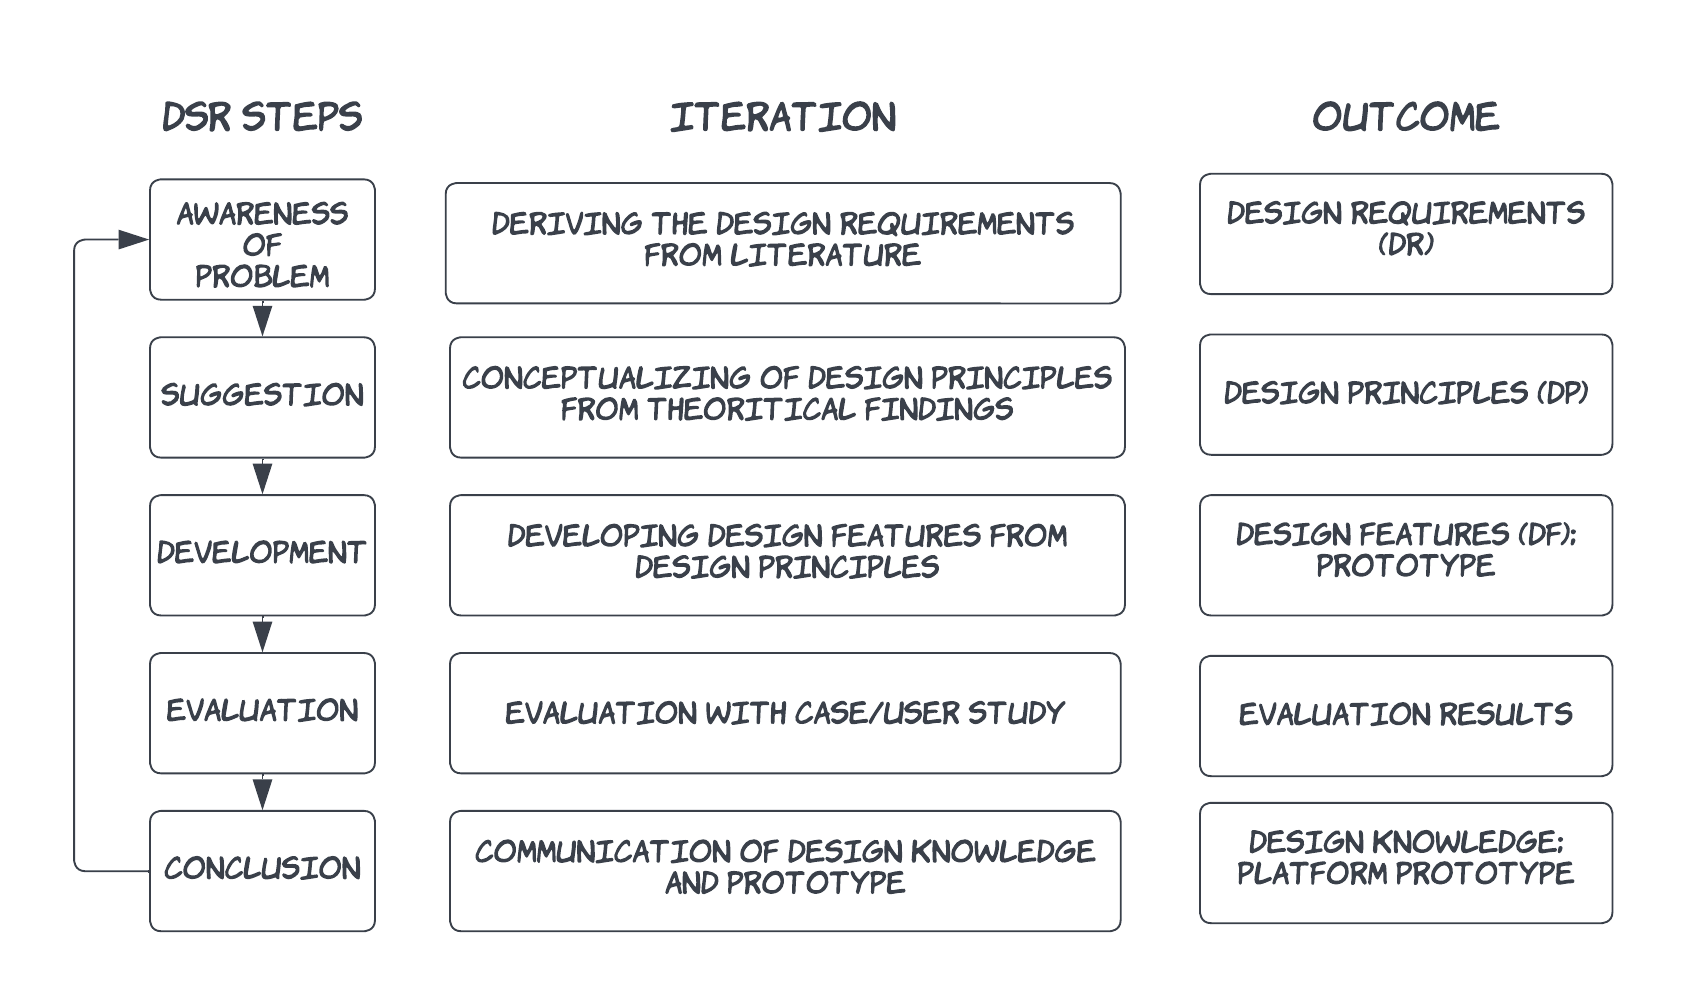
\includegraphics[scale=0.2]{DSRcycle.png}
    \caption{Design Science Research Cycle \cite{paper:designprinciple:vk}}
    \label{intro:fig:dps}
\end{figure}
The process of creating experiments and testing their variants is usually not systematically arranged, creating anomalies, and leading to unsuccessful experiments.
Therefore, this section identifies the research question (RQ) and defines an approach to answer the question.

\paragraph{RQ:} \textit{How to develop a platform suitable for product designers to conduct experiments on UI prototypes, increasing its usability and, simultaneously, independent of developers?}\\

We will conduct a design science research (DSR) study to answer our research question and obtain abstract design knowledge and an implementation tool. 
From the abstracted knowledge, we will obtain some Design Principles (DPs) defined for the whole process of experimentation \cite{paper:designprinciple:vk}.
In this design, the product designers will iteratively validate their prototypes with the users (or the crowds). 
Here, DPs capture and codify that knowledge by focussing on the implementer, the aim, the user, the context, the mechanism, the enactors, and the rationale \cite{paper:designprinciple:gregor}. 
The DPs explain the design information that develops features for software applications.
We propose to use the variation of the cycle of Kuechler and Vaishnavi \cite{paper:designprinciple:vk} consisting of five iteratively conducted steps (see figure \ref{intro:fig:dps}). 
% First, we identify the 
% \texttt{(1) Awareness of the Problem} and provide a
% \texttt{(2) Suggestion of a possible solution}. Next, we work on the 
% \texttt{(3) Development of the software artifact} and conduct an 
% \texttt{(4) Evaluation} of it. Based on the evaluation results, we provide 
% \texttt{(5) Conclusions} \cite{misc:crowdsourcing:sg}.
% From each step of the DSR, we have an iteration cycle and an outcome (e.g., Awareness of the Problem leads to finding Design Requirements, Design Principles (DPs) can be found from the Suggestion of the solution, Development of the software artifact leads to finding the Design Features and the Prototype, etc.) as shown in figure \ref{intro:fig:dps}.
Therefore through the use of DSR, a group of issues is resolved by concentrating on a single issue and abstracting the consequences of the resolution.

\section{Solution Approach}
\label{introduction:section:solution}

To solve the problems mentioned above, the designers should be able to create UI prototypes and experiments on their own on a set of users.
Since we do not have a large set of users for testing the prototypes, we use supervised task-based usability testing \cite{article:dataanalysis:supervisedtest}.
The fundamental principle of task-based usability testing is to have the users attempt to use the prototypes to do certain activities or tasks (e.g., Locate a movie M1) and get feedback (e.g., the time required for the task to be completed by the user).
We propose to use \texttt{Low-code} or \texttt{No-Code} approach to achieve this.
This approach helps to have a UI for the designers to understand, develop, and create experiments and tasks with the software prototypes \cite{paper:lowcode:khorram}.
So, the designers would be able to create the UI prototypes and their variants, assign them to the users in an experiment, get feedback from the users and decide on the best prototype.
At the same time, the low-code has become more accessible for Model-driven development \cite{article:lowcode:modeldriven}.
Therefore, we plan to create models for the UI prototypes and have the feasibility for creating experiments and tasks. 
Because of using the models, it is easier to store the prototypes in the database and conduct experiments with the users. 

\begin{figure}[ht]
    \centering
    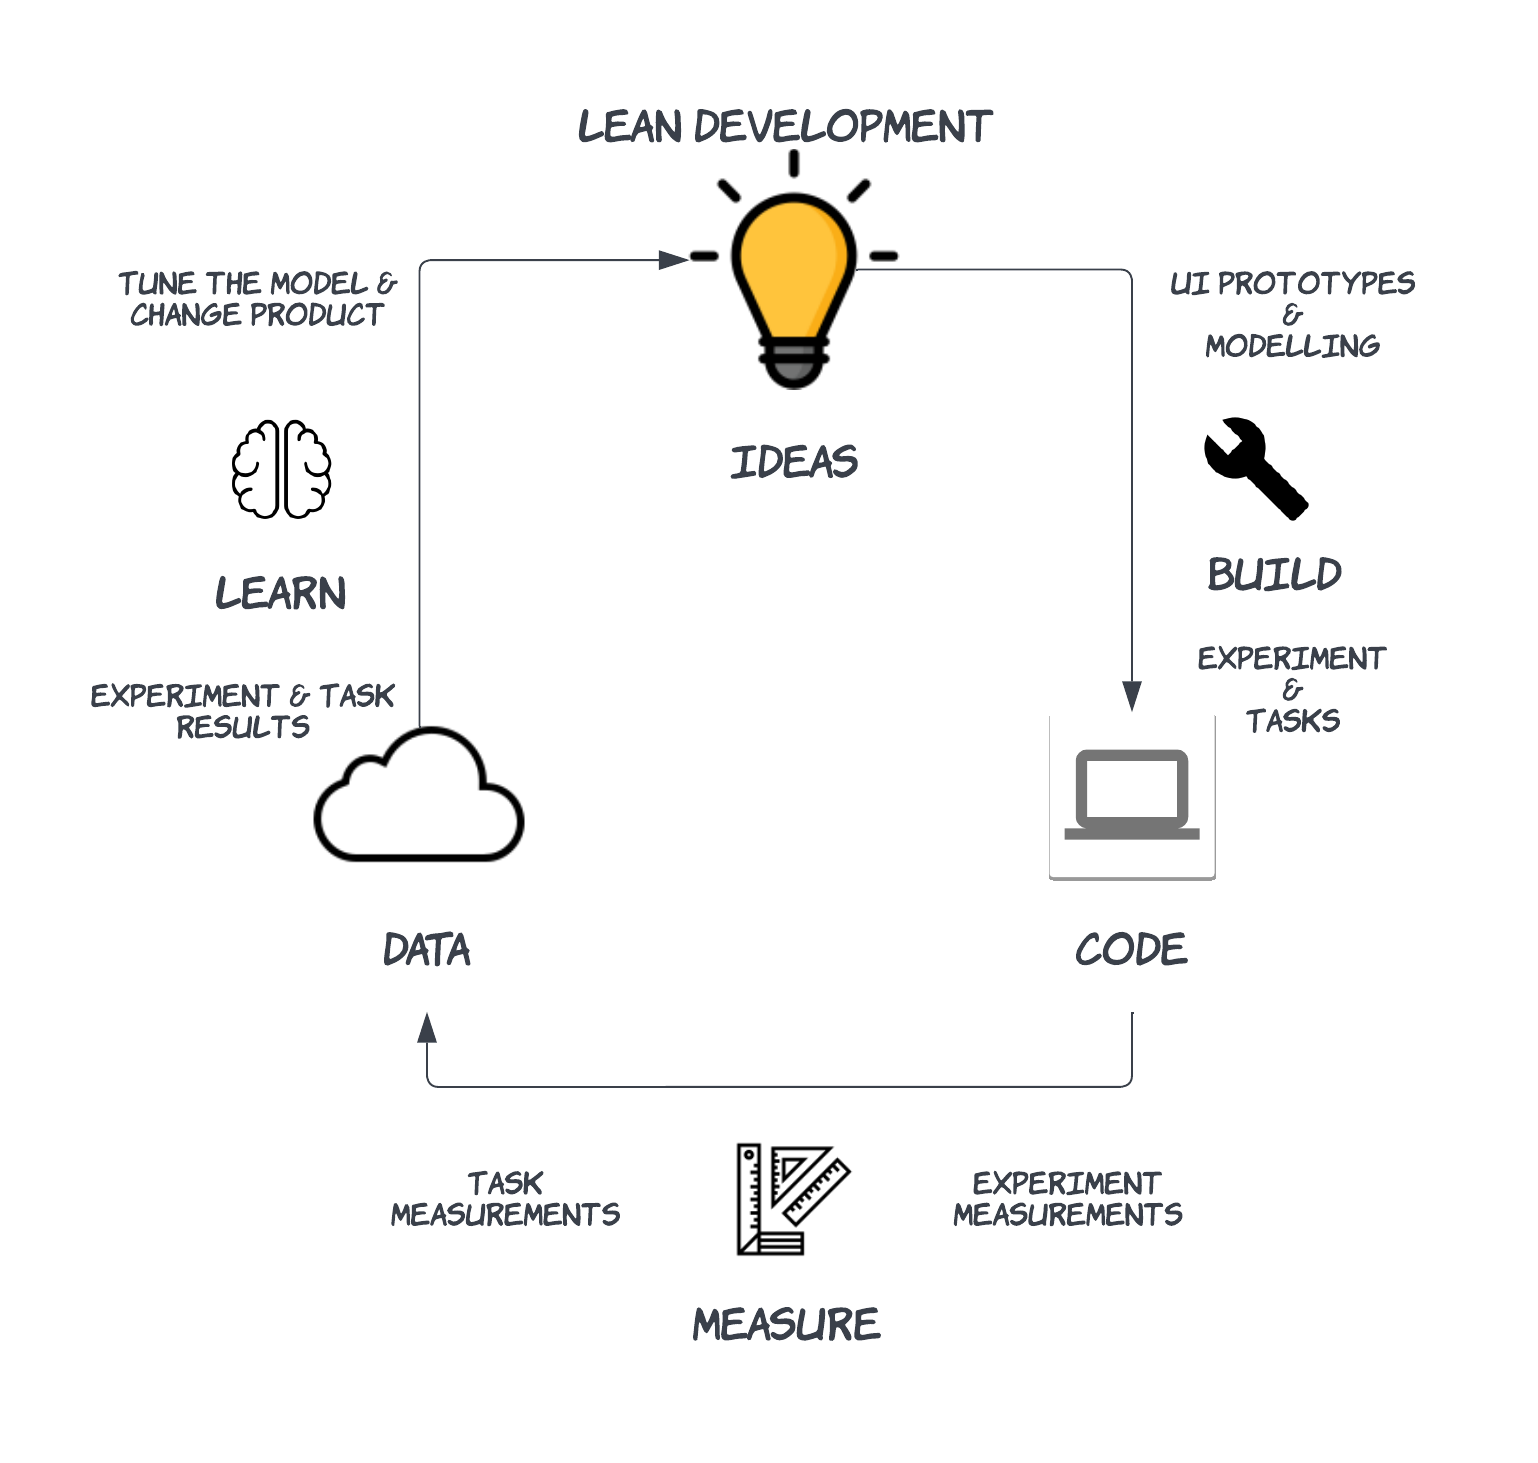
\includegraphics[scale=0.15]{LEAN.png}
    \caption{LEAN Development technique}
    \label{intro:fig:lean}
\end{figure}

In our solution, we use the LEAN development technique (see figure \ref{intro:fig:lean}) for development as it is used to develop customers friendly products \cite{article:lean:hart}.
Using LEAN, the company creates a Minimum Viable Product (MVP) throughout development, tests it with potential customers, and leverages their input to make incremental changes.
While this technique can be used for every product, there are also approaches specific to software products.
LEAN development technique can be divided into a Build, Measure, and Learn cycle. 
In the \texttt{(1) Build} phase, we plan to create the \texttt{UI Prototypes}, \texttt{Models}, \texttt{Experiments}, and \texttt{Tasks} for the users.
In the \texttt{(2) Measure} phase, we plan to assign the Experiments and Tasks to the users and measure the \texttt{Task and the Experiment measurements} and perform some analysis on the data received. 
And finally, in the \texttt{(3) Learn} phase, we display the \texttt{Analyses results}, \texttt{Tune} our models to decide the better variant among the others, and \texttt{Modify} the prototype.
As per the figure \ref{intro:fig:lean}, we complete one cycle of iteration and start a new one with the updated prototype.
%!TEX root = ../../thesis.tex
%*******************************************************************************
%****************************** Background Chapter *********************************
%*******************************************************************************

\chapter{Background}
\ifpdf
    \graphicspath{{Chapters/Background/Figs/}{Chapters/Background/Figs/}{Chapters/Background/Figs/}}
\else
    \graphicspath{{Chapters/Background/Figs/}{Chapters/Background/Figs/}}
\fi
To build the foundation of our approach, we present the usage of crowdsourcing in software development (see section \ref{background:section:crowdsourcing}), UI Prototyping (see section \ref{background:section:uiprototyping}), Low and No code (see section \ref{background:section:lowcode}), Model Based Software Engineering (MBSE) (see section \ref{background:section:mbse}), Task Based Usability Testing (see section \ref{background:section:task}), and Experimental Product Design and define Design Principles (DP) (see section \ref{background:section:experimentproduct}).
%********************************** % Crowdsourcing of Software Products **************************************
\section{Crowdsourcing of Software Products}
\label{background:section:crowdsourcing}
Iterative feedback from potential customers can help improve the development of software products \cite{article:lean:eric}.
To do that, we can use crowdsourcing.
Crowdsourcing refers to outsourcing value-creating activities from a company by an open call to a large, undefined group of users to get feedback \cite{article:crowdsourcing:leimeister}.
The word crowdsourcing is a combination of crowd and outsourcing.
Crowdsourcing often involves less specialized and more generalized groups of participants than outsourcing \cite{article:crowdsourcing:estelles}.
Some advantages of crowdsourcing include lowered costs, improved speed, quality, flexibility, and scalability \cite{article:crowdsourcing:prpic}.
Researchers have used crowdsourcing in many research approaches, including \textit{crowd testing, crowd funding, crowd ideation, crowd logistic, crowd production, crowd promotion,} and \textit{crowd support} over the last few years \cite{article:crowdsourcing:durward}.
In our approach to finding a solution, we focus more on crowd-testing and crowd-ideation.

\paragraph{Crowd Testing:}
The companies use crowd-testing to evaluate different running software products with the users.
A growing trend in software testing is crowd testing, which utilizes the benefits, effectiveness, and efficiency of crowdsourcing and cloud platforms \cite{article:crowdsourcing:latoza}.
Crowd testing is considered when the software is more user-centric: i.e., software with a broad user base whose success is evaluated by user input.
CrowdStudy \cite{article:crowdsourcing:nebeling} is a method that enables developers to assess the usability of their web interfaces using crowd workers from Amazon Mechanical Turk\footnote{Amazon Mechanical Turk: \url{https://www.mturk.com}}.
CrowdCrit \cite{article:crowdsourcing:luther} is another tool that uses Amazon Mechanical Turk to support designers in validating created posters in the form of uploaded images.
Similarly, \textit{Interactive event-flow graphs} and \textit{GUI-level (Graphical User Interface) guidance} \cite{article:crowdsourcing:chen} are the two techniques to increase crowd testers' coverage for GUI using crowd-testing.

\paragraph{Crowd Ideation:}
Design can be infused with creativity by online crowds, but using traditional strategies to harness them, such as large-scale ideation platforms, requires organization and time \cite{article:crowdsourcing:andolina}.
Hence, crowd ideation is used to build new and improved versions of existing software product ideas with the consumers.
Under manipulations of task complexity, idea representation, and procedural guidance, Shixuan Fu et al. \cite{article:crowdsourcing:fu} examine how cognitive load is altered during idea generation and convergence with crowds.
ERICA \cite{article:crowdsourcing:erica} is a tool that uses expert knowledge to validate diverse crowd answers.
Crowdboard \cite{article:crowdsourcing:andolina} is a tool used to engage crowds in real-time brainstorming, concept mapping, and other design processes at an early stage of the design process.
There were, however, no approaches that directly addressed prototype application areas.

%********************************** % UI Prototyping **************************************
\clearpage
\section{UI Prototyping}
\label{background:section:uiprototyping}
\begin{figure}[htbp!]
  \centering    
  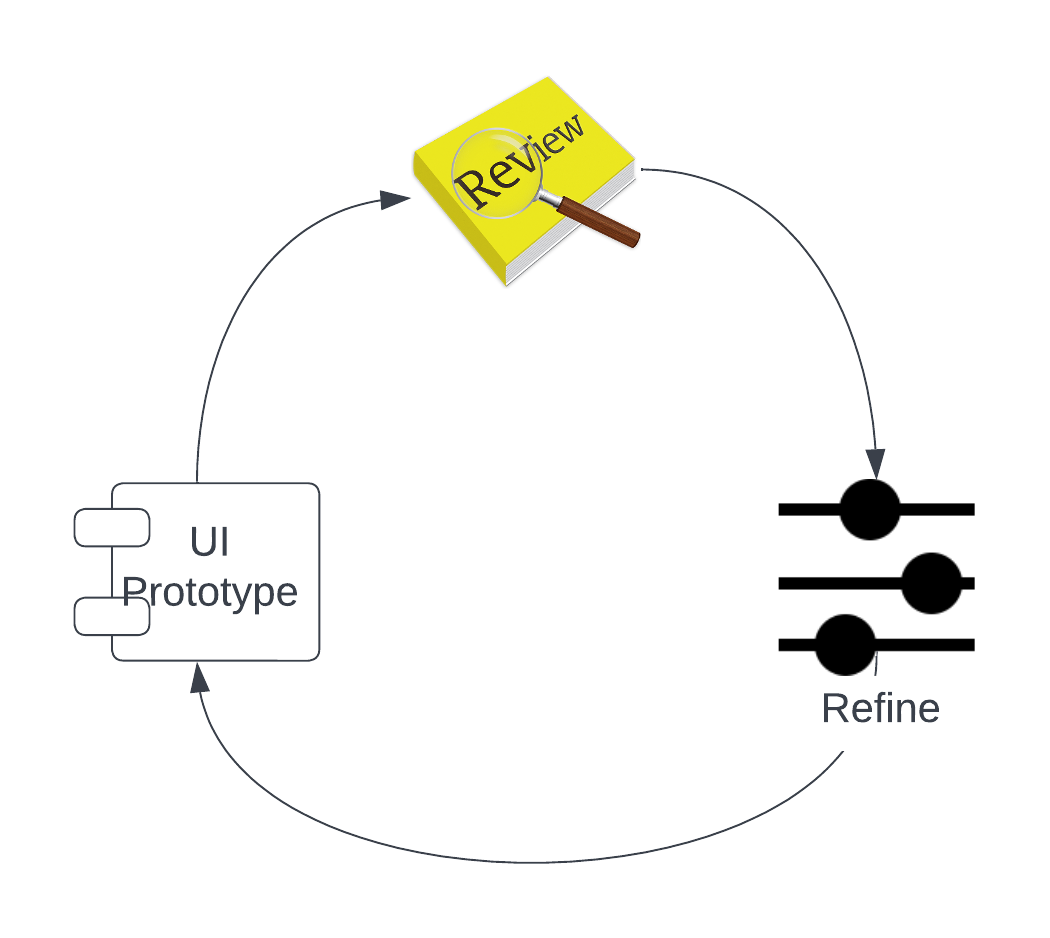
\includegraphics[width=0.6\textwidth]{PrototypingSteps.png}
  \caption[Steps of Prototyping]{Prototyping steps for an iterative development}
  \label{fig:background:stepsPrototyping}
\end{figure}
User Interface (UI) prototyping is an evaluation and testing technique according to User-Centred Design (UCD) methodology since the 1990s \cite{article:prototyping:preece}.
A UI prototype is a mock-up of the User interface.
Before a real product is created, prototypes are used to test the usability and user experience of the interface.
The evaluation of prototypes by users is a fundamental part of all iterative approaches for IT project management, especially agile methodologies \cite{article:prototyping:schwaber}.
And to build an exemplary user interface, iterative refinement must be used: develop a preliminary version of the user interface, test it with people, and make as many revisions as possible \cite{article:prototyping:gould}.
Figure \ref{fig:background:stepsPrototyping} shows a cycle that can be used for the iterative development of prototypes.
The designers start the process by developing the UI prototypes which are reviewed by different stakeholders (e.g., customers, product manager) and from the feedback received the UI prototypes are refined and the cycle is reiterated.
Therefore, designing UI prototypes enables designers and stakeholders to communicate more effectively.

An interactive prototype helps visualize design concepts and communicate new requirements and expectations about a prospective system.
Iterative design requires multiple updates to the design's execution.
\begin{figure}[htbp!]
  \centering
  \begin{subfigure}[b]{0.6\textwidth}
    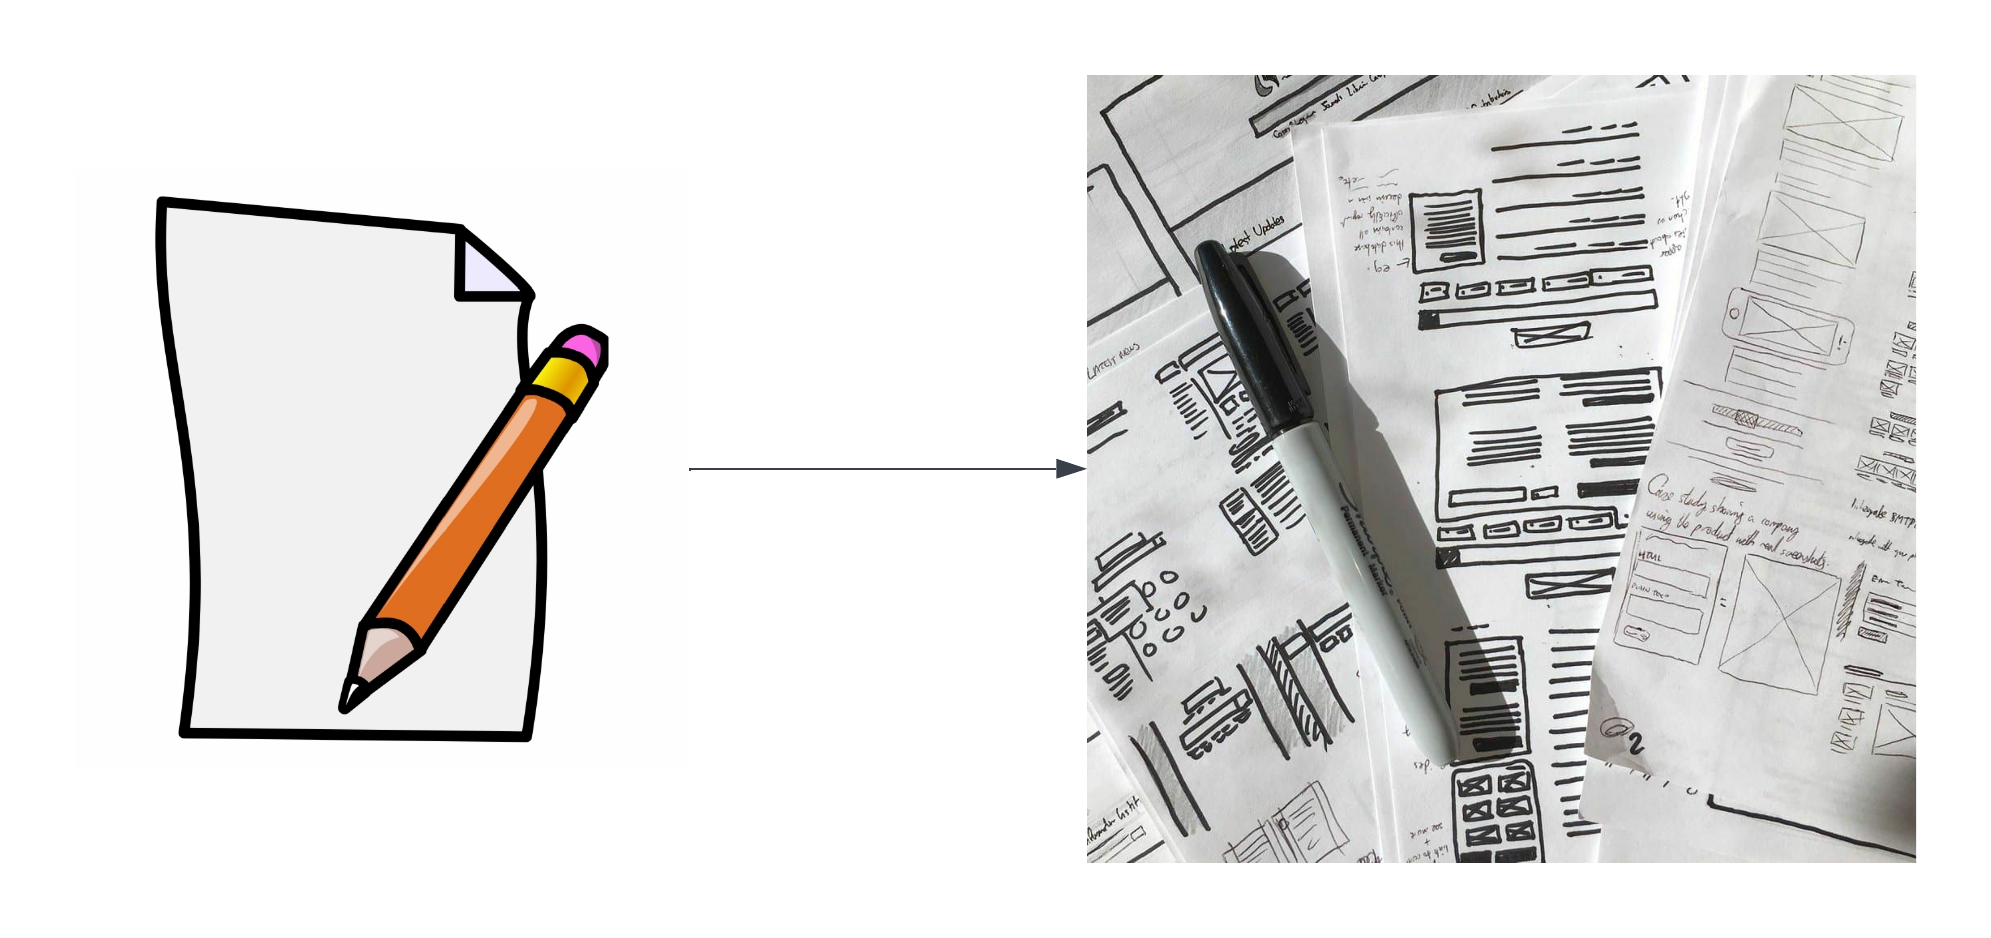
\includegraphics[width=\textwidth]{paperprototyping.png}
    \caption{Sketces and whiteboard for prototyping in initial stages of development}
    \label{fig:background:paperPrototyping}   
  \end{subfigure}             
  \begin{subfigure}[b]{0.5\textwidth}
    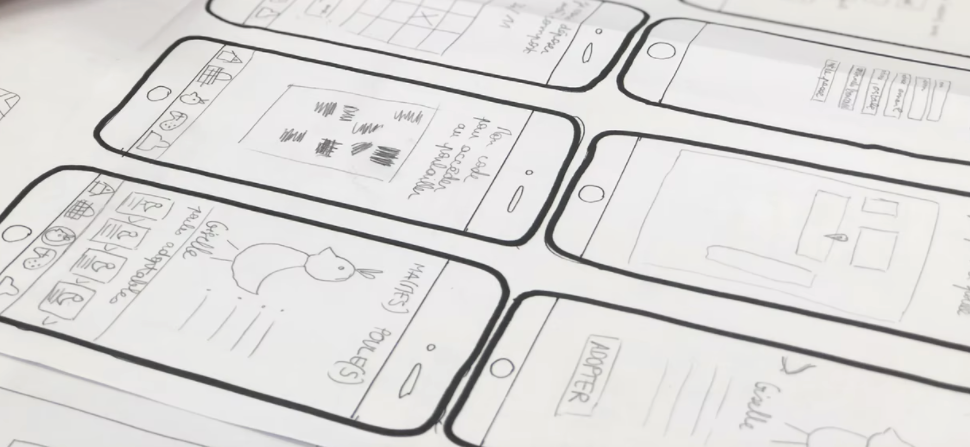
\includegraphics[width=\textwidth]{paperstepsprototypes.png}
    \caption[Paper based prototypes]{Example on how the paper-based prototypes are developed  \cite{misc:prototyping:uxpin}}
    \label{fig:background:paperprototypes}
  \end{subfigure}             
  \caption[Low fidelity prototyping]{Low fidelity prototyping}
  \label{fig:background:main}
\end{figure}
Since developing and updating the entire software system is complex and expensive, prototyping is a crucial technique \cite{article:prototyping:szekely}.
Simultaneously, software prototypes might exclude many requirements, making the software more accessible, smaller, and less expensive to construct and change \cite{article:prototyping:szekely}. 
Similarly, usability testing to validate user requirements and prototype functionality is part of the evaluation process for UI prototypes.
When prototyping is used, there is usually more contact between the designers and users, resulting in fewer usability flaws and corrections at the end of development.
The main difference between a prototype and a software application is that in a prototype the displays are designed images with no additional capabilities to display the design and flow whereas, in a software application the mockups are converted into real UI elements and a flow is available.

From a paper to HTML code, everything could be a prototype.
Jim Rudd et al. \cite{article:prototyping:highlowfidelity} have compared high and low-fidelity prototyping, explaining the advantages and disadvantages.
\textit{Low-fidelity} prototypes (see figure \ref{fig:background:paperPrototyping}) are usually limited functions, with little interaction prototyping effort. They mainly focus on explaining concepts, design alternatives, and screen layouts. 
Storyboard presentations, cards, and proof of concept prototypes come under this category.
UI designers use simple text, lines, and forms to hand-draw concepts. 
Instead of aesthetics, the focus is on speed and a ton of ideas.
To simulate user flows (as shown by figure \ref{fig:background:paperprototypes}), designers lay paper screens on the floor, table, or pinned to a board.
These prototypes emphasize communicating, educating, and informing rather than training, testing, and codification.
The advantages of low-fidelity prototypes are rapid development, lower development cost, addressing issues, and usefulness for a proof-of-concept.
Similarly, the disadvantages include limited error checking, difficulty with usability testing, navigation, flow limitation, etc.
\begin{figure}[htbp!]
  \centering    
  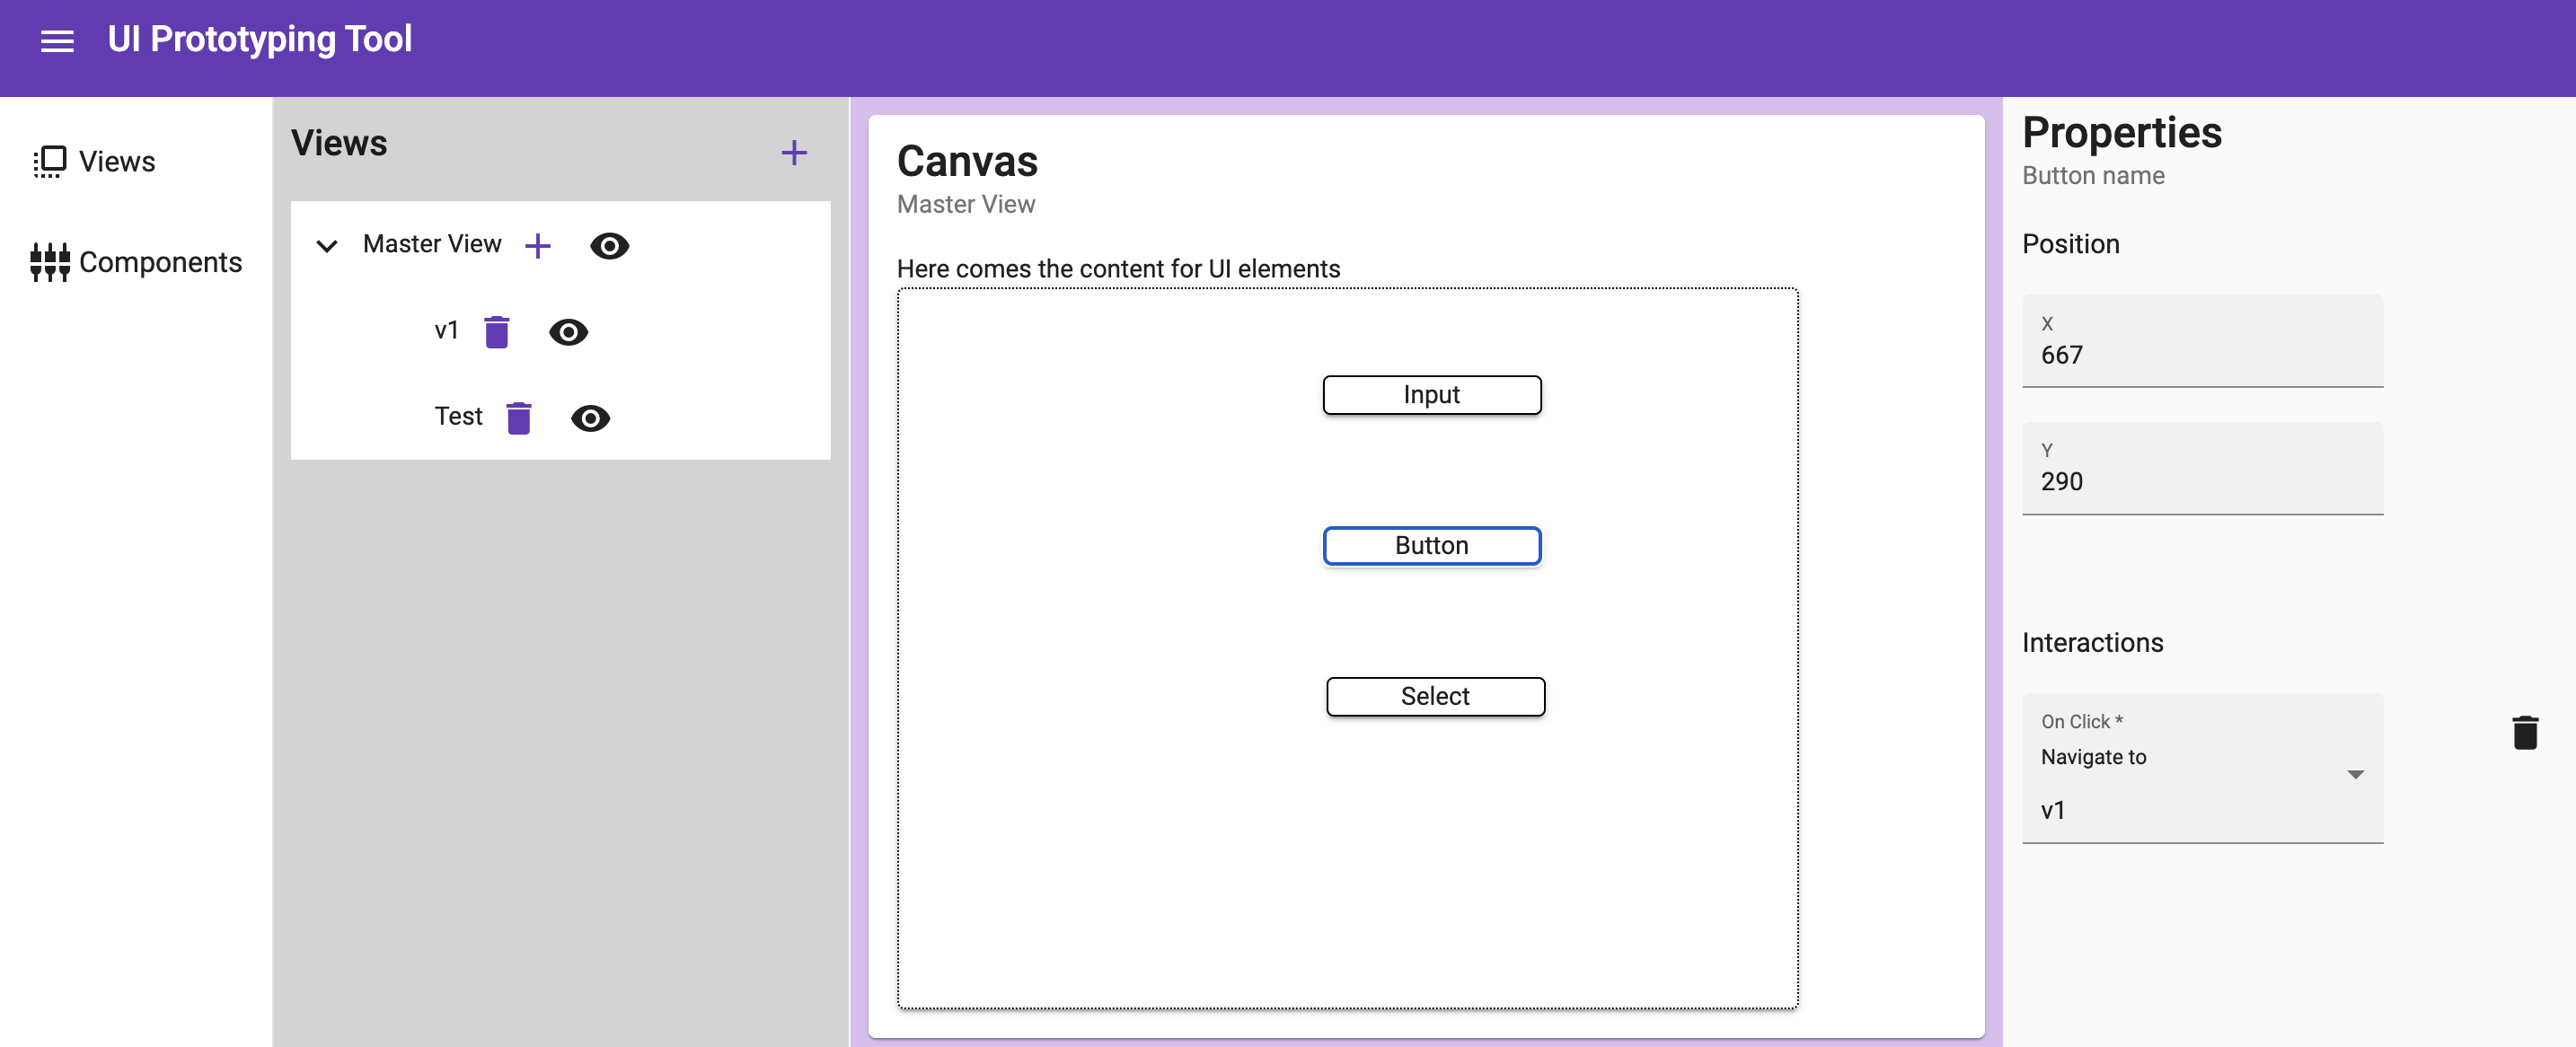
\includegraphics[width=0.9\textwidth]{ui-based-prototyping.png}
  \caption[High Fidelity prototyping]{High Fidelity prototype: Model-based UI Prototyping}
  \label{fig:background:uiPrototyping}
\end{figure}

Contrary to low-fidelity prototypes, \textit{High-fidelity} prototypes (see figure \ref{fig:background:uiPrototyping}) have full functionality and focus on flow, and the user models of the system \cite{article:prototyping:exploratory}.
The users can operate these prototypes, and the developers can collect information from the users through measurements. 
Other advantages of high-fidelity prototypes are that they are user-driven, used for navigation and tests, and can also be served as a marketing tool for attracting potential customers \cite{article:prototyping:highlowfidelity}.\\ \\
\textit{Steps for creating UI Prototypes}:
\begin{itemize}
  \item \textbf{Learn about your consumers' requirements:} Here, our primary goal is to understand the principles that underlie our client's values to better our service to suit their needs. In this step, the design team meets with the product management team and brainstorms to develop some use cases and end-user needs. After the discussions, the team can present the customers to make sure they are on the right track and the design matches their requirements.
  \item \textbf{Sketch out the product:} This is an important step for UI designers. In this step, Low fidelity prototypes can be developed e.g., The design team can create the paper prototypes and start brainstorming on different possible options. Further, the team can create high-fidelity prototypes by using some tools. There are some tools available like Figma\footnote{Figma: \url{https://www.figma.com/}}, Invision\footnote{Invion AG \url{https://www.invisionapp.com/}}, Adobe XD\footnote{Adobe XD: \url{https://www.adobe.com/products/xd.html}}, Axure RP\footnote{Axure RP: \url{https://www.axure.com/}} and many more. Using these tools, the designer can develop some high-fidelity digital prototypes.
  \item \textbf{Develop into Software:} This step includes the software developers and the designers coordinating and developing the software in iterations. The designers would give feedback to the software developers and they would be continuously developing the product.
\end{itemize}

After performing these steps, it is necessary to test if everything is working as expected by the user requirements.
It is necessary to make sure that the product is usable for the end-users and that developers do not miss any important features.
This can be performed in the evaluation phase. 

%********************************** % Low code **************************************
\section{Low Code / No Code Development Platform}
\label{background:section:lowcode}
Low Code is a technique used by developers to help non-developers design and develop software applications using a \textit{Graphical User Interface} (GUI) supported by a \textit{Low Code Development Platform} (LCDP).
Similarly, there is another technique called no code supported by the \textit{No Code Development Platform} (NCDP) \cite{article:nocode:miller}.
Unlike low code, no-code platforms require no programming skills because they offer some prebuild templates for building the apps.
Using the visual user interface and ready-made automatic tools on these application development platforms, it is feasible to create apps relatively quickly. 
These technologies are visual app development methods that speed up app creation by using drag-and-drop editors and pre-built components. 
By allowing software developers to concentrate on challenging coding areas, low code / no code accelerates platform development.
Due to its simplicity, flexibility and low cost, companies have started using this platform to meet the high demands of software development and digitalization.
Low code is a software development method that uses less human coding to enable users to construct and manage programs efficiently \cite{article:nocode:sahina}.
Additionally, it lowers the expenses associated with initial installation, training, distribution, and maintenance \cite{article:nocode:sanchi}.\\ \\
\textit{Main Steps Of \textbf{Low-Code} App Development}
\paragraph*{Building:}
\begin{figure}[htbp!]
  \centering    
  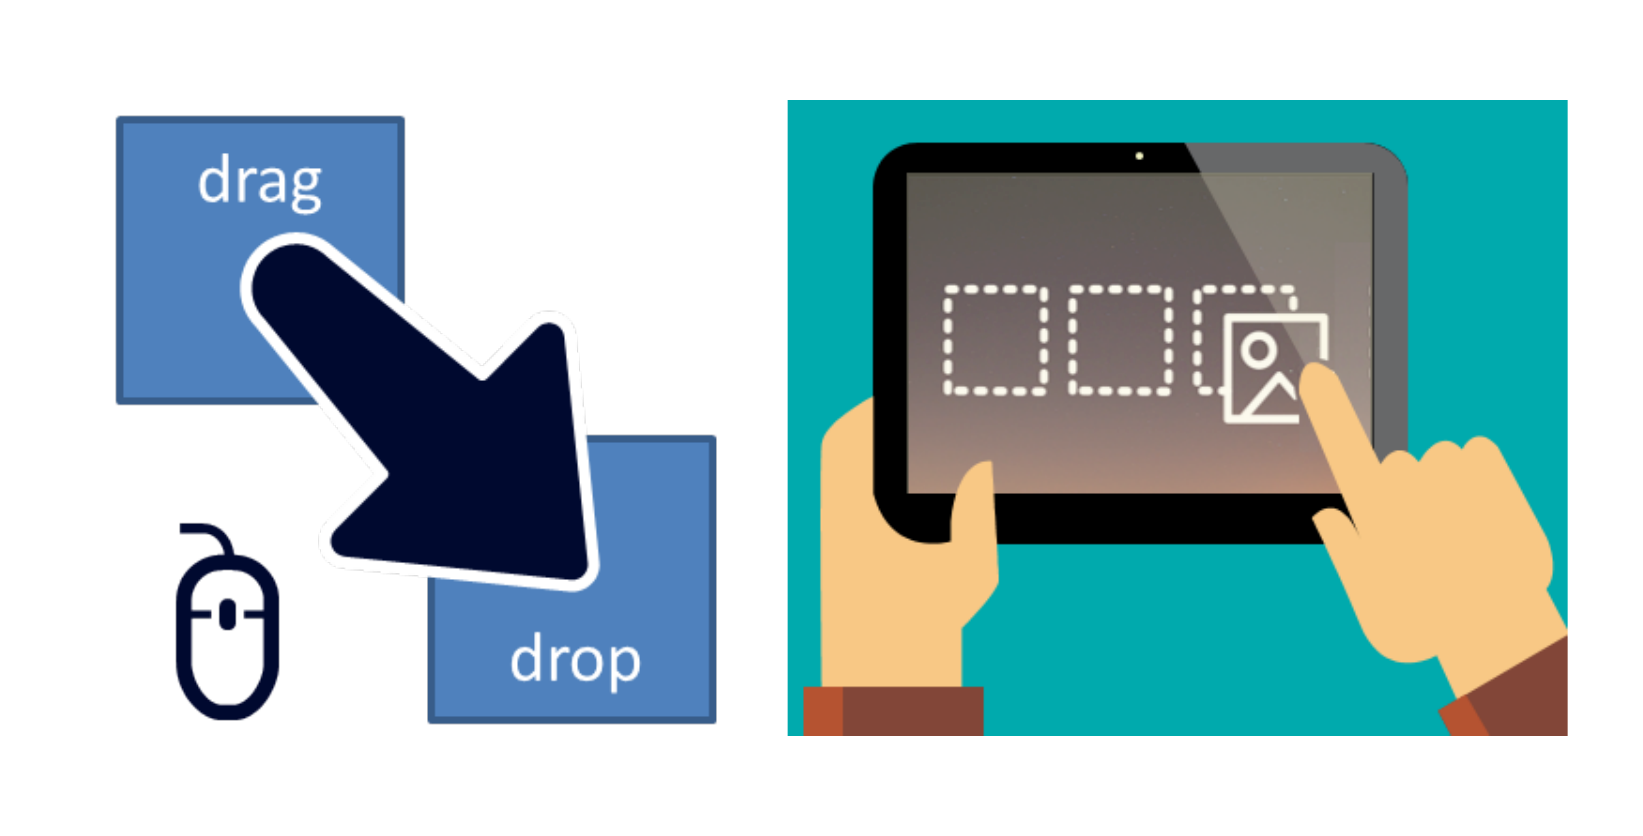
\includegraphics[width=0.7\textwidth]{step1-building.png}
  \caption[Building]{Step 1: Building of Low Code App development}
  \label{fig:background:building}
\end{figure}
In this step (as shown in the figure \ref{fig:background:building}), the platform gives you the freedom to alter the provided code and add hand-written custom code to it to specify more complex features in the app as you create the app step-by-step using visual editors and drag and drop interfaces.
Modules, components, and chart-builders are already incorporated into low-code applications. 
Charts may be used to display data from modules, while modules are used to specify the type of data that will be stored in the app. 
Components and pages provide the type of user experience the app will have.
These platforms also have a provision for the automation of repetitive tasks in the app.
\paragraph*{Testing:}
\begin{figure}[htbp!]
  \centering    
  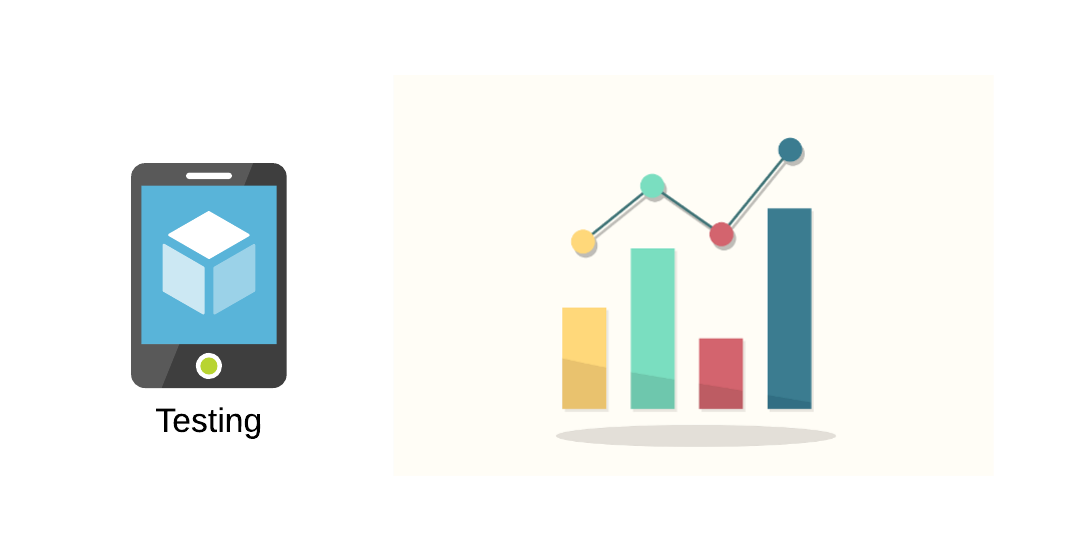
\includegraphics[width=0.9\textwidth]{step2-testing.png}
  \caption[Testing]{Step 2: Testing of Low Code App development}
  \label{fig:background:testing}
\end{figure}
Testing a software application is an important part of the development cycle.
However, the low-code development platform decreases the requirement for testing. 
Pre-build modules and components on low-code platforms are created with a certain level of application security. 
The developers of the low-code platform constantly monitor these modules, and they have previously gone through several unit tests.
But (as shown in figure \ref{fig:background:testing}), we still do need to perform the test on the entire application after integration for scrutiny and this is performed in this step.
\paragraph*{Deploying:}
\begin{figure}[htbp!]
  \centering    
  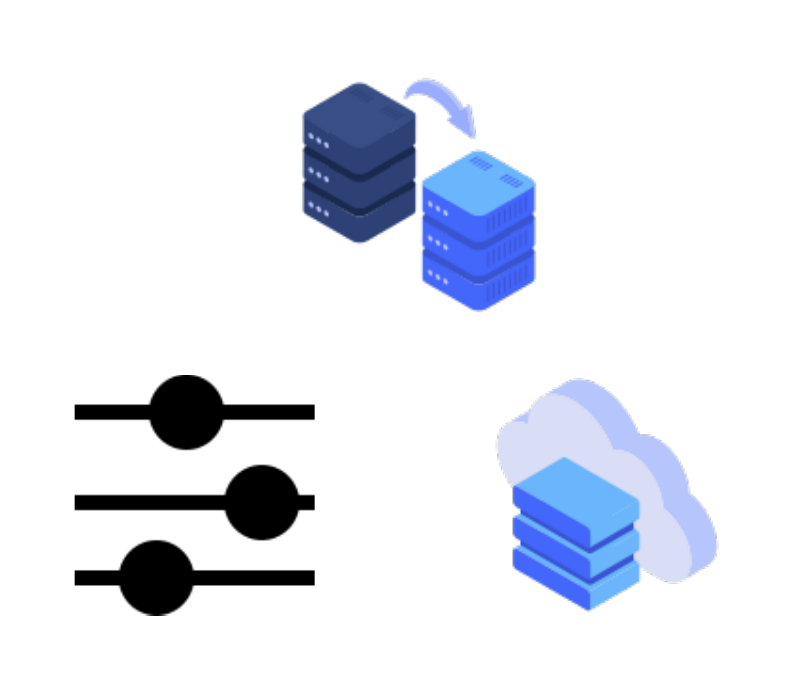
\includegraphics[width=0.7\textwidth]{step3-deployment.png}
  \caption[Testing]{Step 3: Deployment of Low Code App development}
  \label{fig:background:deploying}
\end{figure}
In this step, the application is deployed across apps and to the final users.
In LCDP, the packages for installation, configurations, and application setup are included.
And, the deployment of the app can be done on various services (see figure \ref{fig:background:deploying}) like Cloud-based services.
This means that the LCDP gives freedom to the users in deploying the applications for the customers with just one click.  \\\\
\textit{Some features that make the LCDP or NCDP favorable for development} \cite{article:nocode:sahina, article:nocode:ihirwe, paper:lowcode:cabot}
\begin{itemize}
  \item \textbf{Re-usable components:} LCDP usually contains pre-configured components, modules, logic, templates, and many more that can be customized as per customer requirements. This helps to Build apps with consistency and scalability. Also, the scope for testing decreases as the components of the LCDP is pre-tested for security and performance. 
  \item \textbf{Flexible and Model-driven development:} The drag-and-drop functionality helps developers increase their productivity whereas for citizen developers to build all types of apps. LCDP ensures to have a GUI useful for the non-developers. Therefore, it encourages the stakeholders outside the IT department to participate in development. Low code has become famous in model-driven development. Model-driven development helps to visualize how the app works while it is built.
  \item \textbf{Easy deployment:} This feature ensures that the artifacts are created and the platform is ready to deploy. LCDP has packages that contain various deployment packages (e.g., \texttt{Dockerfile} to deploy on docker\footnote{Docker: \url{https://www.docker.com/}})
\end{itemize}

Additionally, a variety of options are provided for developers with little programming experience, those with coding expertise and seasoned programmers who wish to expand the functionality of the current design \cite{article:nocode:sahina}.

%********************************** % Model-Based Software Engineering **************************************
\section{Model-based Software Engineering}
\label{background:section:mbse}
Model-based Software Engineering (MBSE) refers to maintaining and developing software while reusing existing code.
Similarly, Model-driven software engineering (MDSE) is the term used to cover various techniques for creating software using codified models.
The development of domain-specific languages (DSLs) is becoming essential in language engineering due to the growth in model-driven engineering (MDE) \cite{article:mbse:cuadrado}.
MDSE has become an integral part of developing User interfaces, and they have been named Model-driven User Interfaces (MUIs).
Based on that, adaptive model-driven user interface development systems are developed \cite{article:mbse:akiki}.
In this research, the authors defined twenty properties challenges for the Model-driven User interface and compared some tools that implement these properties.

Companies use different modeling languages to codify the UIs.
Cameleon \cite{article:cameleon:balme} is a framework that divides the UI into several elements to maximize the parts' reusability in various user, platform, and environment situations.
A platform-independent abstract UI, a platform-dependent concrete UI, and a device-dependent final UI are the layers the framework offers to accomplish this.
A standardized modeling language for software product content, abstract UI models, user interactions, and control behavior is Interaction Flow Modeling Language (IFML) \cite{article:ifml:piero}.
As a result, IFML relies on the platform-independent display of the UI that can be utilized on several platforms and devices.

However, these modeling languages do not emphasize offering visual notations to aid non-developers in creating such interfaces. 
A recent method \cite{article:mbse:bexiga} illustrates how to use low-code approaches to close the gap between designers and developers.

%********************************** % Task-based Usability Testing **************************************
\section{Task-based Usability Testing}
\label{background:section:task}
The main focus of usability testing is that seeing someone use an interface is the best approach to determine what functions well and what doesn't. 
Assigning tasks to the accurate number of participants can help determine the quality of the UI and the problems faced by the users. 
Overall, the UI design can be improved using the participants' feedback. 
Task-based usability testing is one way to determine the software's overall usability \cite{article:usability:doesburg} by measuring the percentage of the tasks the users complete.
To observe the participants, they need to be assigned some ``activities'' or \textit{tasks}. 
These tasks need to be some scenarios, not just "\textit{do something}", because it sets the users a stage for \textit{why} they would perform the tasks. 
To get qualitative feedback from the participants, in \cite{misc:usability:tasks}, the authors provide \textit{three good practices} and task-writing tips for designing better task scenarios.
\textit{(1) Make the Task Realistic}.
So, the participants should be able to execute the tasks which could be completed efficiently and with the freedom to make their own choices.
\textit{(2) Make the Task Actionable}.
Here, the participants should be told what they need to do rather than how they would do it.
\textit{(3) Avoid Giving Clues and Describing the Steps}.
The participants should expose the navigation and some features on their own, giving accurate feedback about the interface.
The task scenario example\footnote{Task based usability: \url{https://www.nngroup.com/articles/task-scenarios-usability-testing/}} below sets a target for the participants to locate a movie from our \textit{Videostreamer} app.
\begin{itemize}
  \item[] \textbf{Good and bad example of a task scenario}
  \item \textbf{User goal:} Find a movie. 
  \item \textbf{Bad task scenario:} You should watch a movie on Sunday afternoon. Go to\\ \textit{www.videostreamer.com}, navigate to the Movies page, and find the movie as per the schedule.
  \item \textbf{Good task scenario:} Use \textit{www.videostreamer.com} to find a movie that fits your interest that you'd be interested in watching on Sunday afternoon. 
\end{itemize}
In this example, the \textit{bad} task scenario gives detailed information about the navigation, violating the third tip.

%********************************** % Experimentation **************************************
\section{Experimentation}
\label{background:section:experimentproduct}
Experimental Product Design (EPD) has become integral to optimizing UI and \textit{User Experience (UX)}.
Experimentation helps product teams test out ideas early in the process with real-world consumers rather than settling on a single solution and executing it in the final phase \cite{misc:CE:miklos}.
In this section, we discuss the role that experimentation plays in the software development process and how designers can ``prototype with real data'' to improve the usability of the UI.

\paragraph{Continuous Experimentation:} 
Continuous experimentation (CE) primarily aims to get users' feedback on the software product's evolution.
CE generally uses A/B/n testing in a primary case of comparing two variants, A and B, which are controlled and test variables in an experiment.
With CE, developers make evidence-based decisions to direct the progress of their software by continuously measuring the results of multiple variants performed in an experimental context with actual users \cite{article:CE:ros}.
CE is an extension to the introduction of continuous integration and deployment, and all are summarized as constant software engineering \cite{article:CE:fitzgerald}.

% \clearpage

% \begin{landscape}

% \section{Landscape}
% I can cite Wall-E (see Fig.~\ref{fig:WallE}) and Minions in despicable me (Fig.~\ref{fig:Minnion}) or I can cite the whole figure as Fig.~\ref{fig:animations}


% \begin{figure}
%   \centering
%   \begin{subfigure}[b]{0.3\textwidth}
%     
\includegraphics[width=\textwidth]{minion.png}
%     \caption{Tom and Jerry}
%     \label{fig:TomJerry}   
%   \end{subfigure}             
%   \begin{subfigure}[b]{0.3\textwidth}
%     
\includegraphics[width=\textwidth]{minion.png}
%     \caption{Wall-E}
%     \label{fig:WallE}
%   \end{subfigure}             
%   \begin{subfigure}[b]{0.3\textwidth}
%     
\includegraphics[width=\textwidth]{minion}
%     \caption{Minions}
%     \label{fig:Minnion}
%   \end{subfigure}
%   \caption{Best Animations}
%   \label{fig:animations}
% \end{figure}

% \end{landscape}

%!TEX root = ../thesis.tex
%*******************************************************************************
%****************************** Related Work Chapter **********************************
%*******************************************************************************
\chapter{Related Work}
\label{chap:relatedWork}
\newcolumntype{M}[1]{>{\centering\arraybackslash}m{#1}}
% **************************** Define Graphics Path **************************
\ifpdf
    \graphicspath{{Chapters/Related-work/Figs/}{Chapters/Related-work/Figs/}{Chapters/Related-work/Figs/}}
\else
    \graphicspath{{Chapters/Related-work/Figs/}{Chapters/Related-work/Figs/}}
\fi
In the previous chapter, we explained the evaluation of our solution approach and the tool we developed.
Consequently, in this chapter, we present a comprehensive overview of the related work in two sections. 
The first section (see section \ref{section:related-word:tools}) will discuss the tools commonly used for UI prototyping and UI split testing. 
We will provide an in-depth analysis of the strengths and limitations of each tool and highlight its unique features and functionalities.
The next section (see section \ref{section:related-word:comparison}) focuses on comparing our tool with the existing ones. 
Similarly, in the sections \ref{section:related-word:sota} and \ref{section:related-word:soacomparison} we will discuss some \ac{soa} technologies and compare them. 
We compare different \ac{dr}s we developed in chapter \ref{chap:design} with the other available tools.

\section{Current Tools}
\label{section:related-word:tools}
This section will explore some of the existing softwares or \ac{ra} available in the market.
We have identified some existing tools that are commonly used for UI prototyping and A/B testing.
UX designers widely use these tools to create and test UI prototypes with users. 
Some of these tools are industry-standard and have been around for many years, while others are relatively new.
We will briefly describe each tool's key features and capabilities to provide a comprehensive understanding of the tools we will be comparing.
The comparison will help us identify the gaps and limitations of existing tools and evaluate our tool's uniqueness and innovation. 
Through this section, we aim to provide a comprehensive understanding of the existing tools and technologies and highlight our tool's contributions to the field of UI prototyping and UI split testing.

\paragraph{\ac{ra}1 Figma:} 
Figma\footnote{Website for Figma: \url{https://help.figma.com/hc/en-us/articles/360040314193-Guide-to-prototyping-in-Figma}} is a widely popular user interface design tool designers and design teams use for prototyping, UI design, and collaborative work. 
It has gained popularity due to its versatile features, user-friendly interface, and real-time collaboration capabilities, making it a go-to tool for many designers.
Figma has a broad range of features that allow designers to create complex UI designs easily. 
It includes an extensive library of UI elements, customizable templates, and vector networks to make designing more manageable. 
Additionally, it offers prototyping features that allow designers to simulate complex user interactions and animations, which can help designers validate their decisions quickly. 
Figma is an excellent tool for teams working on the same design project, as it offers real-time collaboration. 
Designers can work together on the same design file, share feedback, and update the design in real-time, making it an efficient and collaborative tool for design teams.

\paragraph{\ac{ra}2 InVision:}
InVision\footnote{Website for InVision: \url{https://www.invisionapp.com/defined/prototype}} is a UI prototyping and collaboration platform that allows designers to create interactive and animated prototypes for web and mobile applications. 
It offers a range of features, including vector-based design tools, advanced animations and interactions, and an extensive library of pre-built UI components.
Its design tools are based on vector graphics, allowing for easy scaling and resizing of elements.
The platform also offers various commenting and annotation tools, making it easy for team members to communicate and collaborate on design decisions.
InVision also offers advanced animation and interaction capabilities, allowing designers to create complex, engaging interactions that simulate real-world user experiences. This feature includes support for animations, transitions, and gestures and the ability to create interactive elements such as buttons, menus, and forms.

\paragraph{\ac{ra}3 Axure:}
Axure\footnote{Website for InVision: \url{https://www.axure.com/prototype}} is another popular prototyping tool used in the industry. 
It is a wireframing and prototyping tool that allows designers to create complex interactions and dynamic content. 
With Axure, designers can create interactive prototypes with conditional logic, animations, and data-driven interactions. 
It also offers collaboration features, which enable teams to work together on the same project in real-time.
Its ability to handle complex logic and conditional interactions sets it apart from many other prototyping tools. 
However, the learning curve can be steep, and there may be better choices for designers looking for a quick and easy way to create simple prototypes.
Finally, Axure offers integrations with other design and collaboration tools, which can benefit teams using multiple tools in their workflow.

\paragraph{\ac{ra}4 Adobe XD:}
Adobe XD\footnote{Website for Adobe XD: \url{https://www.adobe.com/products/xd/learn/get-started-xd-prototype.html}} is a popular tool for designing and prototyping digital products, including websites, mobile apps, and other interactive experiences. 
It is widely used by UX designers, product managers, and other professionals in the design industry. 
One of the key features of Adobe XD is its ability to create interactive prototypes. 
With XD, designers can create clickable, interactive mockups of their designs, allowing them to test user flows and interactions before writing any code. 
These prototypes can also be shared with stakeholders and users for feedback.
In addition to prototyping, it is possible to integrate external plugins to conduct A/B testing in Adobe XD. 
One such plugin is UserTesting, which allows designers to recruit participants and set up tasks for A/B testing directly within Adobe XD. 

\paragraph{\ac{ra}5 Proto.io:} 
Proto.io\footnote{Website for Adobe XD: \url{https://proto.io/developers/}} is a powerful UI prototyping tool widely used in the industry. 
It offers a variety of features to create interactive prototypes, including the ability to add animations, transitions, and gestures. 
Proto.io provides an intuitive drag-and-drop interface and supports multiple platforms, including iOS, Android, and the web.
One of the standout features of Proto.io is its ability to simulate the final product. 
This feature allows designers to create prototypes that look and feel like the final product, providing a more realistic user experience. 
Proto.io also provides advanced collaboration features, making sharing and collaborating on designs with team members and stakeholders easy.
Another key feature of Proto.io is its ability to create A/B tests. The tool offers a dedicated A/B testing feature, which allows designers to create multiple versions of a design and test them against each other. The tool also provides detailed analytics and user feedback, helping designers make informed design decisions.

\paragraph{\ac{ra}6 Google Optimize}
Google Optimize\footnote{Website for Google Optimize: \url{https://developers.google.com/optimize/devguides/experiments?technology=ga4}} is an A/B testing and personalization tool developed by Google. 
It is a cloud-based tool that can help businesses optimize their website or app by creating and running experiments. 
Google Optimize has a user-friendly interface allowing users to create experiments without coding knowledge. 
One of the key features of Google Optimize is the ability to create A/B tests with different variations of a website or app. 
Users can set up experiments to test various elements of their website or app, such as headlines, images, or calls to action. 
Google Optimize also allows users to create multivariate tests that test multiple elements simultaneously.
Another important feature of Google Optimize is the ability to create personalization experiments. 
Users can create targeted experiences for specific audiences based on location, behavior, or demographics. 
This allows businesses to create more relevant and engaging experiences for their users.
Google Optimize also integrates with other Google products, such as Google Analytics, allowing users to analyze experiment results and gain insights into user behavior. 
Additionally, Google Optimize supports third-party integrations.

\paragraph{\ac{ra}7 VWO}
VWO\footnote{Website for VWO: \url{https://help.vwo.com/hc/en-us/articles/360021171954-How-to-Create-an-A-B-Test-in-VWO-}} (Visual Website Optimizer) is another popular tool for A/B testing and conversion rate optimization. 
It is a cloud-based platform that enables users to run experiments on their websites or mobile apps to improve the user experience and increase conversions.
VWO offers a variety of features for A/B testing, including split URL testing, heatmaps, session recordings, surveys, and personalization. 
Users can create and run experiments with a simple WYSIWYG\footnote{Website for WYSIWYG: \url{https://www.howtogeek.com/752396/what-is-a-wysiwyg-editor/}} editor or use custom code for more advanced experiments.
VWO also provides a powerful targeting engine that allows users to target specific segments of their audience, such as first-time visitors, returning visitors, or users who have abandoned a shopping cart. 
This targeting engine helps to ensure that experiments are relevant to the user and are more likely to lead to a positive outcome.

\paragraph{\ac{ra}8 Convertize}
Convertize\footnote{Website for Convertize: \url{https://docs.convertize.io/docs/how-to-do-ab-testing/}} is a website optimization tool that provides a wide range of features for A/B testing, personalization, and targeting. 
It enables marketers to create and test multiple websites or landing page versions to determine which design, layout, or content performs best for their target audience.
Convertize offers a visual editor allowing users to create different variations of their website without coding skills. 
Users can drag and drop elements, such as images, text, and buttons, to create different versions of their websites, which can then be tested against each other.
One of the unique features of Convertize is its AI-powered Autopilot mode, which allows users to automate the optimization process. With Autopilot, Convertize automatically adapts the website to each visitor by personalizing the content, design, and layout to maximize conversions.
Another notable feature of Convertize is its SmartEditor, which uses a library of pre-built templates and machine learning algorithms to recommend changes to website elements, such as headlines, images, and CTAs, that will likely improve conversions.

\paragraph{\ac{ra}9 Freshmarketer}
Freshmarketer\footnote{Website for Freshmarketer: \url{https://support.freshmarketer.com/en/support/solutions/folders/50000000186/page/3}} is a comprehensive conversion optimization suite that offers a range of tools to help businesses optimize their website and improve their online performance. 
It allows users to create and execute A/B tests, track visitor behavior, and gather customer feedback from a single platform. 
Freshmarketer's A/B testing tool enables users to create multiple webpage variants and test them against each other to determine which is most effective at achieving a specific goal, such as increasing conversions or decreasing bounce rates. 
The platform also offers advanced targeting options to help users deliver personalized experiences to particular audience segments.
In addition to A/B testing, Freshmarketer offers a range of other optimization tools, including heatmaps, session replays, and form analytics, to help users gain deeper insights into visitor behavior and identify areas for improvement. 
Freshmarketer's customer feedback tools, such as surveys and polls, allow users to collect valuable customer insights and use that feedback to inform future optimization efforts. 

\paragraph{\ac{ra}10 Zoho PageSense}
Zoho PageSense\footnote{Website for Zoho Pagesense: \url{https://help.zoho.com/portal/en/kb/pagesense/run-a-b-and-split-url-tests/create-and-launch-a-test/articles/a-b-test}} is a web optimization tool designed to help businesses optimize their website's user experience, increase visitor engagement, and boost conversions. 
Zoho PageSense offers many features to help businesses optimize their website, including A/B testing, heatmaps, funnel analysis, and more.
With Zoho PageSense's A/B testing feature, businesses can create multiple variations of their website pages and test them against each other to determine which performs best. 
Zoho PageSense offers a visual editor that allows users to create and edit website page variations without requiring coding knowledge.
In addition to A/B testing, Zoho PageSense offers heatmaps, allowing businesses to visualize how users interact with their website pages. 
This feature enables companies to identify areas of their website that are not performing well and make data-driven decisions to improve the user experience.

\clearpage
\section{Comparison of tools}
\label{section:related-word:comparison}
In comparing the different tools based on the \ac{dr}s (see table \ref{table:related:work:comparision}), we can see that only some tools fulfilled all the \ac{dr}s. 
\ac{ra}5 and \ac{ra}6 fulfilled the most \ac{dr}s, with \ac{ra}5 fulfilling five out of ten \ac{dr}s and \ac{ra}6 fulfilling six out of ten DRs.
For \textit{Heterogeneous Users (DR1)}, only \ac{ra}5, \ac{ra}6, \ac{ra}9, and \ac{ra}10 fulfilled this requirement completely. Most of the other tools only partially fulfilled this requirement.
Most tools fulfilled this requirement for \textit{Iterative Design (DR2)}, but some only partially fulfilled it.
For \textit{Easy Development (DR3)}, \ac{ra}1, \ac{ra}2, \ac{ra}3, \ac{ra}4, and \ac{ra}5 fulfilled this requirement. 
The rest of the tools did not fulfill it.
For \textit{Integrate Data Models (DR4)}, only \ac{ra}3 fulfilled this requirement completely. 
Most of the other tools only partially fulfilled this requirement.
For \textit{Classified UI Variants (DR5)} and \textit{Conduct Split Tests (DR6)}, \ac{ra}5, \ac{ra}6, \ac{ra}7, \ac{ra}8, \ac{ra}9, and \ac{ra}10 fulfilled this requirement, but the rest of the tools still need to.

\begin{table}[htbp!]
  \centering
  \begin{tabular}{| M{2em} || M{2em} | M{2em} | M{2em} | M{2.1em} | M{2.1em} | M{2.1em} | M{2em} | M{2em} | M{2em} | M{2.2em} |}
  \hline 
  \multicolumn{11}{|c|}{\textbf{Comparison between different Tools}} \\ 
  \hline
  \textbf{Tool} & \textbf{DR1} & \textbf{DR2} & \textbf{DR3} & \textbf{DR4} & \textbf{DR5} & \textbf{DR6} & \textbf{DR7} & \textbf{DR8} & \textbf{DR9} & \textbf{DR10} \\
  \hline
  \ac{ra}1 & \priority{50} & \priority{100} & \priority{100} & \priority{50} & \priority{0} & \priority{0} & \priority{0} & \priority{50} & \priority{0} & \priority{50} \\
  \hline
  \ac{ra}2 & \priority{50} & \priority{100} & \priority{100} & \priority{50} & \priority{50} & \priority{50} & \priority{0} & \priority{50} & \priority{0} & \priority{50} \\
  \hline
  \ac{ra}3 & \priority{50} & \priority{100} & \priority{100} & \priority{100} & \priority{0} & \priority{0} & \priority{0} & \priority{50} & \priority{0} & \priority{50} \\
  \hline
  \ac{ra}4 & \priority{50} & \priority{100} & \priority{100} & \priority{50} & \priority{50} & \priority{50} & \priority{0} & \priority{50} & \priority{50} & \priority{50} \\
  \hline
  \ac{ra}5 & \priority{100} & \priority{50} & \priority{100} & \priority{0} & \priority{100} & \priority{100} & \priority{50} & \priority{100} & \priority{50} & \priority{100} \\
  \hline
  \ac{ra}6 & \priority{100} & \priority{100} & \priority{0} & \priority{0} & \priority{100} & \priority{100} & \priority{50} & \priority{100} & \priority{100} & \priority{100} \\
  \hline                                   
  \ac{ra}7 & \priority{50} & \priority{100} & \priority{0} & \priority{0} & \priority{100} & \priority{100} & \priority{50} & \priority{100} & \priority{50} & \priority{100} \\
  \hline
  \ac{ra}8 & \priority{50} & \priority{50} & \priority{0} & \priority{0} & \priority{100} & \priority{100} & \priority{50} & \priority{100} & \priority{50} & \priority{50} \\
  \hline
  \ac{ra}9 & \priority{100} & \priority{100} & \priority{0} & \priority{0} & \priority{100} & \priority{100} & \priority{100} & \priority{100} & \priority{50} & \priority{50} \\
  \hline
  \ac{ra}10 & \priority{100} & \priority{100} & \priority{0} & \priority{0} & \priority{100} & \priority{100} & \priority{100} & \priority{100} & \priority{50} & \priority{100} \\
  \hline
  \hline
  \multicolumn{1}{|c}{Legend:} & \multicolumn{3}{c}{No Fulfillment (\priority{0})} & \multicolumn{3}{c}{Partial Fulfilment (\priority{50})} & \multicolumn{4}{c|}{Complete Fulfilment (\priority{100})} \\
  \hline
  \end{tabular}
  \caption[Comparison between different approaches]{Table comparing different \ac{ra}s against \ac{dr}s}
  \label{table:related:work:comparision}
\end{table}

For \textit{Conduct User Tasks (DR7)}, only \ac{ra}9 and \ac{ra}10 fulfilled this requirement completely. The rest of the tools only partially fulfilled this requirement or did not fulfill it.
Similarly, for \textit{Collect User Feedback (DR8)}, most tools partially fulfilled this requirement, except for \ac{ra}5, \ac{ra}6, \ac{ra}7, \ac{ra}9, and \ac{ra}10 which fulfilled this requirement completely.
For \textit{Aggregated Feedback (DR9)}, most tools only partially or still need to fulfill this requirement. 
Only \ac{ra}5 fulfilled this requirement completely.
For \textit{Improvement (DR10)}, most of the tools only partially fulfilled this requirement or still need to fulfill it. 
Only \ac{ra}5, \ac{ra}6, \ac{ra}7, and \ac{ra}10 fulfilled this requirement completely.
Overall, each tool had its strengths and weaknesses in fulfilling the different DRs, and no tool could completely fulfill all our DRs.

\clearpage

\section{State-of-the-art technologies (SOAT)}
\label{section:related-word:sota}
This section explores some \ac{soa} or cutting-edge technologies for UI prototyping and A/B testing of UI. 
UX designers widely use these technologies to create and test UI prototypes with users. 
This section aims to provide a comprehensive understanding of the existing \ac{soa} and highlight our technology's contributions to UI prototyping and UI split testing using the \ac{dr}s. 
We will provide a comprehensive overview of each technology's key features and capabilities to understand the these technologies we will compare comprehensively. 
The comparison will help us identify the gaps and limitations of existing technologies and evaluate our technology's uniqueness and innovation.

\paragraph{RA11 Rapid software prototyping approach}
L. Luqi et al. \cite{paper:prototyping:luqi} propose a rapid software prototyping methodology that utilizes a visual design tool and object-oriented technology. 
The authors argue that traditional software development methodologies need to provide adequate support for rapidly creating prototypes that can be used to communicate design ideas with stakeholders. 
To address this issue, they propose a framework that combines a visual design tool for creating user interfaces with object-oriented technology to build functional prototypes quickly. 
The authors demonstrate the effectiveness of their methodology through a case study, which shows that the proposed framework can significantly reduce the time and effort required to develop functional prototypes.

\paragraph{RA12 Continuous Prototyping approach}
Lukas Alperowitz et al. \cite{misc:prototyping:lukas} propose a continuous prototyping approach to bridge the gap between design and development in continuous software engineering. 
The authors argue that traditional software development methodologies must provide adequate support for continuous prototyping, a critical aspect of iterative design and development processes. 
To address this issue, they propose a framework that enables designers and developers to continuously prototype and refine their design ideas as part of the software development process. 
The authors demonstrate the effectiveness of their approach through a case study, which shows that continuous prototyping can significantly improve the quality and speed of software development and increase stakeholder satisfaction.

\paragraph{RA13 Data-Driven Approaches to User Interface Design}
Pimenov et al. \cite{misc:data-driven:pimenov} present a case study on data-driven approaches to user interface design. 
The authors argue that traditional user interface design methods rely on expert opinions and intuition, which may not always reflect the actual needs and preferences of users. 
To address this issue, they propose a data-driven approach that utilizes user feedback and analytics to inform design decisions. 
The authors demonstrate the effectiveness of their approach through a case study, which shows that data-driven design can lead to significant improvements in user satisfaction and task completion rates. 
The paper provides insights into the potential of data-driven approaches to user interface design and highlights the importance of incorporating user feedback and analytics in the design process.

\paragraph{RA14 A Tool for Online Experiment-Driven Adaptation}
Ilias Gerostathopoulos et al. \cite{misc:experiment:ilias} propose a tool for online experiment-driven adaptation. 
The authors argue that traditional software development approaches must provide adequate support for online experimentation and transformation, which are critical for improving the UX and achieving business goals. 
To address this issue, they propose a framework that enables developers and designers to create and deploy online experiments that can be used to test and optimize different aspects of the software system. 
The authors demonstrate the effectiveness of their approach through a case study, which shows that the proposed tool can significantly improve the effectiveness of online experimentation and adaptation. 
The paper provides insights into the potential of experiment-driven transformation to improve software systems and highlights the importance of incorporating data-driven approaches in software development.

\paragraph{RA15 A promising tool for customer value evaluation}
Peitsa Hynninen et al. \cite{misc:abtest:marjo} propose using A/B testing as a promising tool for evaluating customer value. 
The authors argue that traditional methods of customer value evaluation, such as surveys and focus groups, may not provide accurate or reliable results due to biases and limitations. 
To address this issue, they propose the use of A/B testing, which is a randomized experiment that compares the effectiveness of two or more alternatives in achieving a specific goal. 
The authors demonstrate the effectiveness of A/B testing through a case study, which shows that A/B testing can provide valuable insights into customer preferences and behavior. 
The paper provides insights into the potential of A/B testing as a tool for customer value evaluation. 
It highlights the importance of incorporating data-driven approaches in marketing and customer experience strategies. 

\clearpage
\section{Comparison}
\label{section:related-word:soacomparison}
In our chapter on design chapter \ref{chap:design}, we identified 10 DRs for the development of effective user interfaces. To evaluate the state-of-the-art research (SOAT) based on these DRs, we analyzed five studies, namely SOAT11, SOAT12, SOAT13, SOAT14, and SOAT15 (see table \ref{table:related:work:soacomparision}).
\begin{table}[htbp!]
  \centering
  \begin{tabular}{| M{3em} || M{2em} | M{2em} | M{2em} | M{2.1em} | M{2.1em} | M{2.1em} | M{2em} | M{2em} | M{2em} | M{2.2em} |}
  \hline 
  \multicolumn{11}{|c|}{\textbf{Comparison between different \ac{soa}}} \\ 
  \hline
  \textbf{Tool} & \textbf{DR1} & \textbf{DR2} & \textbf{DR3} & \textbf{DR4} & \textbf{DR5} & \textbf{DR6} & \textbf{DR7} & \textbf{DR8} & \textbf{DR9} & \textbf{DR10} \\
  \hline
  \ac{soa}11 & \priority{0} & \priority{100} & \priority{100} & \priority{50} & \priority{0} & \priority{0} & \priority{0} & \priority{0} & \priority{0} & \priority{100} \\
  \hline
  \ac{soa}12 & \priority{0} & \priority{100} & \priority{100} & \priority{100} & \priority{50} & \priority{0} & \priority{0} & \priority{50} & \priority{0} & \priority{100} \\
  \hline
  \ac{soa}13 & \priority{50} & \priority{50} & \priority{50} & \priority{100} & \priority{0} & \priority{0} & \priority{50} & \priority{100} & \priority{100} & \priority{50} \\
  \hline
  \ac{soa}14 & \priority{100} & \priority{50} & \priority{0} & \priority{0} & \priority{50} & \priority{100} & \priority{50} & \priority{100} & \priority{50} & \priority{50} \\
  \hline
  \ac{soa}15 & \priority{100} & \priority{50} & \priority{0} & \priority{0} & \priority{100} & \priority{100} & \priority{50} & \priority{50} & \priority{50} & \priority{50} \\
  \hline
  \hline
  \multicolumn{1}{|c}{Legend:} & \multicolumn{3}{c}{No Fulfillment (\priority{0})} & \multicolumn{3}{c}{Partial Fulfilment (\priority{50})} & \multicolumn{4}{c|}{Complete Fulfilment (\priority{100})} \\
  \hline
  \end{tabular}
  \caption[Comparison between different \ac{soa} approaches]{Table comparing different \ac{soa}s against \ac{dr}s}
  \label{table:related:work:soacomparision}
\end{table}

\ac{soa}11 fulfilled DR2, DR3, and DR10, partially fulfilled DR4, and failed to fulfill DR1, DR5, DR6, DR7, DR8, and DR9. 
\ac{soa}12 fulfilled DR2, DR3, DR4, and DR10, partially fulfilled DR5 and DR8, and failed to fulfill DR1, DR6, DR7, DR9. 
\ac{soa}13 partially fulfilled DR1, DR2, DR3, DR7, DR8, and DR10, fulfilled DR4 and DR8, and failed to fulfill DR5 and DR6. 
\ac{soa}14 fulfilled DR1, DR6, and DR8, partially fulfilled DR2, DR5, DR7, and DR9, and failed to fulfill DR3 and DR4. 
Finally, \ac{soa}15 fulfilled DR1, DR5, DR6, and DR10, partially fulfilled DR2, DR7, DR8, and DR9, and failed to fulfill DR3 and DR4.

Overall, we observed that none of the \ac{soa}s fully fulfilled our identified DRs. 
However, \ac{soa}15 achieved the most DRs, with four fulfilled and four partially fulfilled, while \ac{soa}11 and \ac{soa}12 each achieved three fulfilled DRs. 
Our analysis demonstrates the need for continued research in developing effective user interfaces that fulfill all identified DRs.
%!TEX root = ../thesis.tex
%*******************************************************************************
%****************************** Design Chapter *********************************
%*******************************************************************************

\chapter{Design}

\ifpdf
    \graphicspath{{Chapters/Design/Figs/}{Chapters/Design/Figs/}{Chapters/Design/Figs/}}
\else
    \graphicspath{{Chapters/Design/Figs/}{Chapters/Design/Figs/}}
\fi

%********************************** % Design Principles **************************************
\section{Design Principles}

%********************************** % Build **************************************
\section{Build}

%********************************** % Measure **************************************
\section{Measure}

%********************************** % Learn **************************************
\section{Learn}

%!TEX root = ../../thesis.tex
%*******************************************************************************
%****************************** Solution Implementation Chapter *********************************
%*******************************************************************************

\chapter{Solution Implementation}

\ifpdf
    \graphicspath{{Chapters/Implementation/Figs/}{Chapters/Implementation/Figs/}{Chapters/Implementation/Figs/}}
\else
    \graphicspath{{Chapters/Implementation/Figs/}{Chapters/Implementation/Figs/}}
\fi
In the previous chapter, we displayed an overview design of our approach.
Consequently, the solution implementation chapter of this thesis presents the details of how the proposed system was developed and implemented.
Firstly, we define some \ac{df} (see section \ref{implementation:section:designfeatures}) that focus on designing and developing new artifacts, methods, or systems.
It begins with a description of the system's architecture (see section \ref{implementation:section:architecture}), including the major components and their interactions.
Next, the description of the technology stack and development tools is explained (see section \ref{implementation:section:technologies}).
The chapter includes a detailed explanation of the critical features and functionality of the system and the processes used in frontend implementation (see section \ref{implementation:section:frontend}), database implementation (see section \ref{implementation:section:database}) backend implementation (see section \ref{implementation:section:backend}), and the software tool (see section \ref{implementation:section:tool}). 
Finally, the chapter discusses the challenges encountered during the implementation process and the lessons learned (see section \ref{implementation:section:challenges}). 
Through this chapter, readers will understand how we brought the proposed solution to reality and its potential for real-world applications.

\section{Platform Design Features (DFs)}
\label{implementation:section:designfeatures}
\ac{dsr} aims to produce a tangible outcome, such as a new software tool, a process improvement, or a theoretical framework.
It often involves multiple cycles of design, evaluation, and redesign, allowing for constant improvement of the artifact.
Since we perform the \textit{first} iteration of the cycle, we derive the features of our software tool using the \ac{df}s.
In this section, we translate each \ac{dp}s (we defined in chapter \ref{chap:design}) into a set of \ac{df}s that we can directly implement into the tool or solution approach and we describe the \ac{df}s for each of the derived \ac{dp}s.
\clearpage
Based on the \textbf{\ac{dp}1: User Variety}, the key features of our solution approach for the \ac{ui} prototyping tool will include registration for diverse users using a registration form (\textit{\ac{df}1}) and user management, i.e., features that enable team members to create and manage user accounts (\textit{\ac{df}2}), assign different levels of access and permissions (\textit{\ac{df}3}). 

Based on the \textbf{\ac{dp}4: Pre-Designed Interactive UI Elements}, the privileged user would be able to prototype using the features of our solution approach, which includes the creation of different screens (\textit{\ac{df}4}) and reusable \ac{ui} elements using a drag and drop interface (\textit{\ac{df}4}). The tool also provides a feature to add custom data. i.e., creating data models table (\textit{\ac{df}5}), revising structures of data model table (\textit{\ac{df}6}), adding and deleting data from the table (\textit{\ac{df}7}).

Based on the \textbf{\ac{dp}2: Split Tests}, the privileged user would be able to create A/B tests or UI experimentation using the features of our solution approach, which includes creating and modifying the experiments (\textit{\ac{df}8}), creating and updating the UI variants (\textit{\ac{df}9}), and modifying the variants' prototypes such that each variant has a unique view (\textit{\ac{df}10}). 

Based on the \textbf{\ac{dp}5: User tasks Refinement}, the privileged user would be able to create Tasks for the participants using the features of our solution approach, which includes creating tasks for participants depending on the data model (\textit{\ac{df}11}) and independent of data models (\textit{\ac{df}12}), and assign the task to the experiments (\textit{\ac{df}13}).

Based on the \textbf{\ac{dp}6: Qualitative Analysis}, the privileged user would be able to do qualitative analysis on the participants using the features of our solution approach, which includes creating the custom qualitative questionnaire (\textit{\ac{df}14}) with options in the answering formats like Scale based, i.e., the participants will have to choose from options 1 to 10 (\textit{\ac{df}15}) and open-ended questions, i.e., the participants will have the freedom to answer whatever they think (\textit{\ac{df}16}). Similarly, the participants will answer these questions after finishing the tasks with a modal appearing with different questions (\textit{\ac{df}17}). 

Based on the \textbf{\ac{dp}7: Quantitative Analysis}, the privileged user would be able to do quantitative analysis on the participants using the features of our solution approach, which includes collecting the task data feedback, i.e., collecting the time taken to finish the task, number of unsuccessful attempts, the path taken by the users to complete the task, etc. (\textit{\ac{df}18}), and aggregating these feedback data (\textit{\ac{df}19}. 

Based on the \textbf{\ac{dp}8: Diversity in Analysis}, the privileged user would be able to compare the statistics using the features of our solution approach, which includes showing the results of the experiment (\textit{\ac{df}20}), combining qualitative and quantitative analysis of each variant (\textit{\ac{df}21}), and a graphical view to see the results (\textit{\ac{df}22}). 

Based on the \textbf{\ac{dp}3: Continuous Design}, the solution approach would provide features including LEAN development cycle (\textit{\ac{df}23}). The privileged user should be able to update the original prototype with the results from the experiment (\textit{\ac{df}24}) for continuous improvement. 

Based on the \textbf{\ac{dp}9: Modeling}, the solution approach would provide features for creating the models (\textit{\ac{df}25}) useful for persisting data in the database and updating them (\textit{\ac{df}26}) with the results of the experiments.

\section{Technologies Used}
\label{implementation:section:technologies}
We have created a software tool that allows us to test the features (\ac{df}s) and underlying principles of the developed DFs with actual users.
To test our solution approach, we developed a rapid prototyping tool for the first cycle of our \ac{dsr}. 

The implementation of our \textit{UI Prototyping Tool with Experimentation (UPTE)} platform uses various technologies.
Our UI prototyping tool was developed using Angular\footnote{A framework of javascript: \url{https://angular.io/}}, Loopback\footnote{A framework of the NodeJS \url{https://loopback.io/}}, and MongoDB\footnote{A non-relational database \url{https://www.mongodb.com/}}.
Angular is a JavaScript framework used for building web-based applications.
It provides comprehensive tools for creating dynamic and responsive UI components and handling user interactions.
With angular, we are using several other UI components which are available on Node package manager (npm)\footnote{NPM: \url{https://www.npmjs.com/}}.

Loopback is a Node.js\footnote{NodeJS: \url{https://nodejs.org/en/}} framework used for building RESTful APIs. 
It provides an intuitive interface for creating API endpoints and managing data persistence. 
Loopback's support for various data sources, including relational and NoSQL databases, makes it a versatile choice for web applications. 
We connect our database using the data managers provided by the loopback framework.
The framework's ability to generate API documentation and testing tools simplifies our development process.

MongoDB is a NoSQL document-oriented database used for storing unstructured data. 
We store our prototyping tool's data using a JSON\footnote{What is JSON: \url{https://developer.mozilla.org/en-US/docs/Glossary/JSON}} format in an unstructured manner.
It provides a scalable and flexible solution for managing volumes of data. 
MongoDB's support for automatic sharding and replication ensures high availability and fault tolerance. 
The database's dynamic schema and rich query language make it easy to adapt to changing data requirements.

By leveraging these technologies, our UI prototyping tool delivered a powerful and user-friendly interface while ensuring efficient data retrieval and storage.
Based on these technologies, we build a microservice architecture explained in the next section so that our \ac{dp}s and \ac{df}s can be easily implemented. 

\section{Solution Architecture}
\label{implementation:section:architecture}

\section{Frontend Implementation}
\label{implementation:section:frontend}

\section{Database Schema}
\label{implementation:section:database}

\section{Backend Implementation}
\label{implementation:section:backend}

\section{Software Tool}
\label{implementation:section:tool}

\section{Encountered Challenges and Lessons Learnt}
\label{implementation:section:challenges}
%!TEX root = ../thesis.tex
%*******************************************************************************
%****************************** Evaluation Chapter *********************************
%*******************************************************************************

\chapter{Evaluation}
\label{chap:evaluation}
In the previous chapter, we explained the implementation of our tool. 
Based on that, in this chapter, we will discuss the details of the evaluation process, including the user case study (see section \ref{evaluation:section:casestudy}), experimental design (see section \ref{evaluation:section:design}), execution (see section \ref{evaluation:section:execution}), analysis (see section \ref{evaluation:section:analysis}), and interpretation (see section \ref{evaluation:section:interpretation}) of the results. 
For the setup, we recruited participants from Paderborn University.
\ifpdf
    \graphicspath{{Chapters/Evaluation/Figs/}{Chapters/Evaluation/Figs/}{Chapters/Evaluation/Figs/}}
\else
    \graphicspath{{Chapters/Evaluation/Figs/}{Chapters/Evaluation/Figs/}}
\fi

\section{User Case Study}
\label{evaluation:section:casestudy}
To evaluate the effectiveness of our approach, we conducted a case study that involved recruiting participants, developing prototypes, and working on user scenarios. 
We recruited 15 participants who are students at Paderborn University. 
The case study is based on the evaluation stage of the first cycle of our DSR (as discussed in section \ref{introduction:section:research}). 
In conducting and reporting our case study research, we followed the established guidelines of Runeson and Höst \cite{eval:guidlines:runeson} (see figure \ref{evaluation:fig:casestudy}) to increase the quality of the study outcomes. 
These guidelines helped ensure our research was rigorous, transparent, and credible. 
By adhering to these guidelines, we aimed to provide a detailed and comprehensive account of our case study, enabling others to replicate our research and build upon our findings.
This case study also aims to develop the RQ as explained in the next section.

\clearpage
\section{Experimental Design}
\label{evaluation:section:design}
In this section, as per Runeson and Höst, we first define the objective, case study, research questions, and the methods we follow to complete the evaluation.

\paragraph{Objective:}
The objective of the user case study was to evaluate a \ac{poc} tool for creating and testing UI designs. 
The goal was to assess the tool's ability to generate UI prototypes, create split or A/B tests, and collect participant feedback to select the best variant.

\paragraph{Case Study:}
The case study involved a user scenario where John, a UX designer, was responsible for designing the UI for a new movie-streaming app. John used the \ac{poc} tool to create UI prototypes and perform split tests to select the best variant.

\paragraph{Research Questions (RQs):}
For the case study, we defined a couple of research questions. \\
\textbf{RQ1:} Can a \ac{poc} tool be used to prototype the UI of a new movie-streaming app and create split or A/B tests to select the best variant of the app's interface design? \\
\textbf{RQ2:} What feedback can be gathered from participants to evaluate the effectiveness of different app interface design variants?

\begin{figure}[ht]
    \centering
    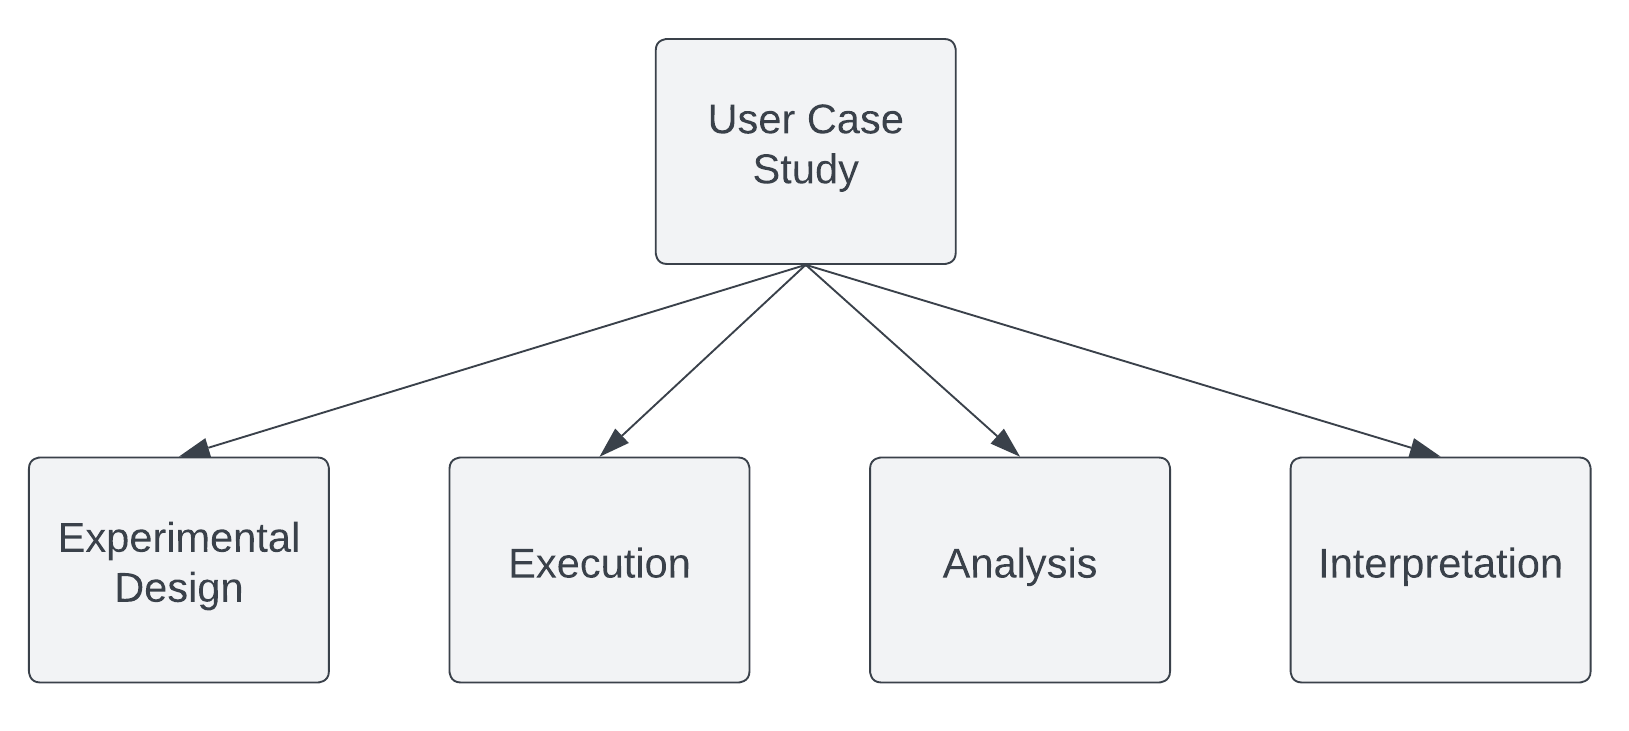
\includegraphics[scale=0.25]{case-study.png}
    \caption{User Case Study for Analysis}
    \label{evaluation:fig:casestudy}
\end{figure}

\paragraph{Method:}
For the User Case Study, we aimed to recruit diverse participants from different courses enrolled at Paderborn University to ensure a wide range of perspectives and experiences on UI prototyping and UI Experimentation. 
We wanted to include individuals with varying levels of experience in prototyping and user scenario development, from beginners to experts. 
To recruit participants, we used Doodle\footnote{Website for Doodle: \url{https://doodle.com/}}, an online tool for setting up the appointment, and a Line survey\footnote{Website for the survey: \url{https://umfragen.uni-paderborn.de/admin/}} hosted by our university for creating the questionnaire.

We developed a user scenario that required participants to use our UI prototyping tool hosted on the Paderborn University server. 
Therefore to access our tool, the participants needed to turn on the VPN\footnote{Website for University Paderborn VPN config: \url{https://imt.uni-paderborn.de/vpn-zugang/}} provided by the University. 
We also examined them using an open BigBlueButton\footnote{Website for BBB: \url{https://open-bbb.uni-paderborn.de/}} video conference session. 
We also considered the ethical clarifications by informing the participants that we were not recording the video conference session and that the survey was anonymous to ensure their privacy and encourage honest feedback while mentioning our data collection and storage strategy.

After using the tool, participants were asked to answer a questionnaire in the survey to provide qualitative and quantitative feedback for our tool and the \ac{dp}s we developed. 
The questionnaire was designed to evaluate the usability, effectiveness, and overall satisfaction with our tool. 
We also asked for suggestions for improvement and gathered additional comments and feedback from the participants to gain a deeper understanding of their experiences.

\clearpage
\section{Execution}
\label{evaluation:section:execution}
In this section, we explain the execution of our user case study in detail. 
First, we explain the planning phase of the execution and then explain the methodology of how we conducted the survey.

\paragraph{Planning:}
Before conducting the user case study, we carefully planned the experimental design to ensure the validity and reliability of our results.
First, we defined a hypothesis to be tested. We wanted our POC tool to fulfill the Design principles and validate the DPs. 
To achieve this, we developed a user scenario that involved the participants using our tool to create a prototype and conduct a user scenario. 
We recruited diverse participants enrolled in various courses at Paderborn University, with varying experience in prototyping and user scenario development.
To recruit participants for our case study, we shared a Doodle link via different communication channels, such as email and social media. 
The Doodle link contained the necessary information about the study, including the purpose, duration, and requirements. 
It also offered different time slots for the participants, ensuring that the survey could accommodate a diverse group of participants with varying schedules. 
This method helped us efficiently reach out to potential participants and allowed them to select a time that suited them best.

Secondly, we used the Lime survey, hosted on the Paderborn University server, to conduct a survey questionnaire to collect qualitative and quantitative feedback from the participants. 
The questionnaire was divided into three sections. 
The first section contained the \ac{sus} questionnaire, a widely used and reliable tool for measuring the usability of software systems. 
This section aimed to collect quantitative feedback from the participants regarding the usability of our prototype tool. 
The second section contained questions about the design principles we proposed in our thesis. 
This section aimed to collect participants' ratings and opinions on the effectiveness and feasibility of the design principles. 
The third section contained open-ended questions to gather participants' qualitative feedback and suggestions for improving our prototype tool and the \ac{dp}s. 
We used the Lime survey to facilitate the data collection process and to ensure anonymity and privacy for the participants.

\paragraph{Methodology:}
The methodology of our user case study involved using a proof of concept tool accessible via UPB VPN that combined qualitative and quantitative data collection and analysis techniques. The participants were then asked to conduct a user scenario using our tool while being observed through an open BBB video conference session.
The scenario was that John, a UX designer, was creating a new movie-streaming app and wanted to prototype different UI designs and conduct split tests to select the best variant. 
The study was conducted in several phases.

In the first phase, John explored the tool and generated an example movie streaming prototype using the headstart button. He then added new movies to the prototype using the data model feature.
In the second phase, John created split tests for different app interface versions. 
He used the tool's A/B testing feature to create two versions of the app's view screen and changed the UI to make some changes in the variant's prototype.
In the third phase, John created tasks for participants to complete and gather feedback on the app's interface. 
He also created a set of questionnaires, including open-ended and scale-based questions, to collect qualitative data from participants.
In the fourth phase, John recruited participants or used dummy users generated from the tool to test the experiments and monitor the results. 
After completing the experiment, John navigated to the experiments page and analyzed the statistics to determine which version of the app's interface was more effective.
Based on the feedback from the usability tests and questionnaires, John iterated on the app's design and updated the prototype in the tool. 
Overall, the execution of the experiment involved prototyping, split testing, task creation, and feedback gathering to design and improve the movie-streaming app's interface. 
An example prototype, created by one of the user participants is shown in Appendix \ref{appendix:three:caseStudy}.

\clearpage
\section{Analysis}
\label{evaluation:section:analysis}
After collecting the data through LimeSurvey and the tool, we analyzed the feedback and results to draw insights and conclusions about the effectiveness of our research questions and the software tool we designed. 
We also examined the qualitative feedback from the participants to gain a deeper understanding of their preferences and needs. 
Next, we explain the qualitative and quantitative analysis of the data collected from the participants in detail.

\paragraph{Quantitative analysis}
\begin{figure}[ht]
    \centering
    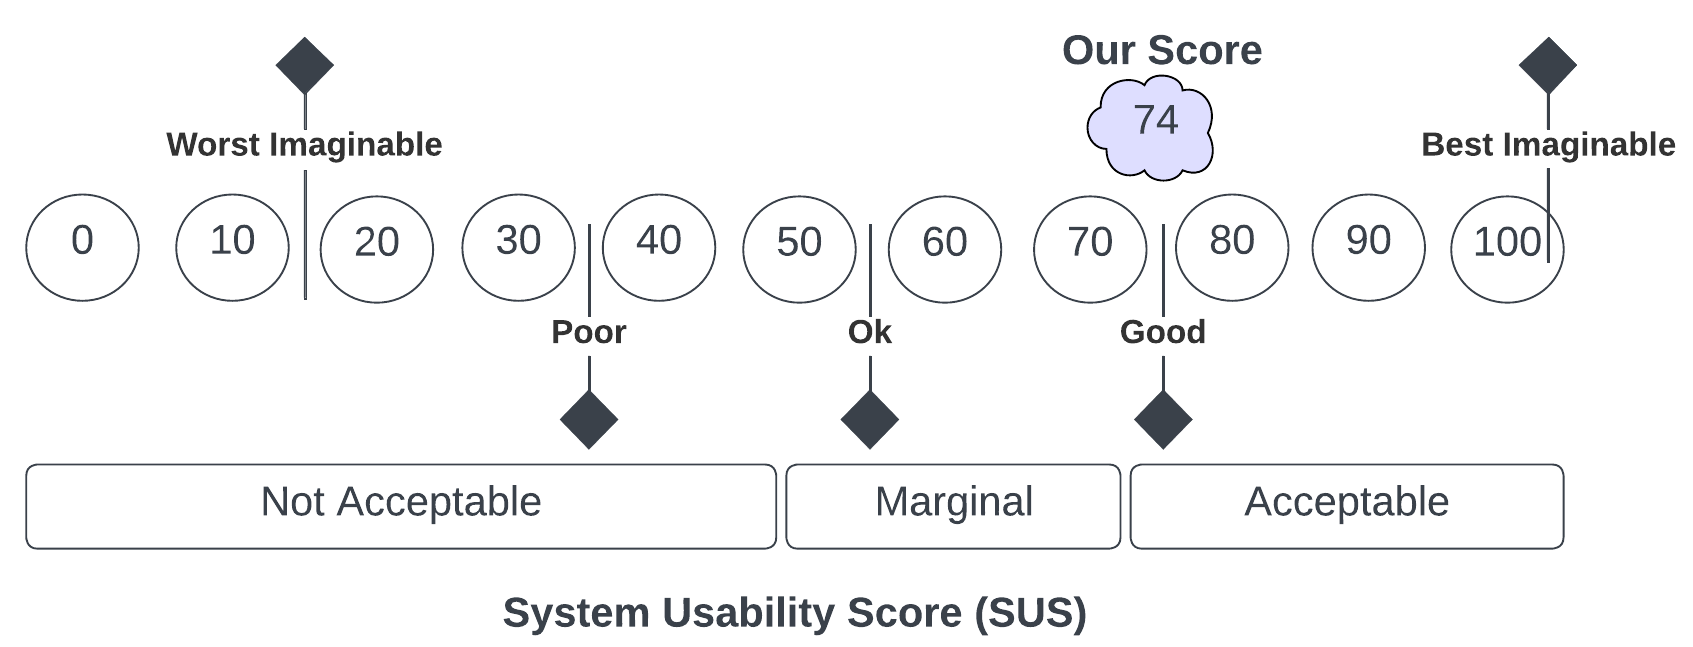
\includegraphics[scale=0.25]{SUS.png}
    \caption{System Usability score (SUS) of our tool}
    \label{evaluation:fig:sus}
\end{figure}
In the first part of the quantitative section of our analysis, we utilized the \ac{sus} to gather feedback on the usability of our tool. 
The \ac{sus} is a widely used and well-established questionnaire for assessing the usability of a system. 
It consists of 10 statements that participants rate on a 5-point scale from 1 (strongly disagree) to 5 (strongly agree). 
The scores from each report are then combined and transformed to create a final \ac{sus} score ranging from 0 to 100.
After administering the \ac{sus} questionnaire to our participants, we computed the average score to obtain a quantitative measure of the usability of our tool. 
We also analyzed the individual scores for each statement to identify areas where the tool performed well and where improvements could be made. 
It allowed us to gain insights into the strengths and weaknesses of our tool from a quantitative perspective. 
It provided a basis for making data-driven decisions about improving the tool's usability. 
Our analysis of the \ac{sus} survey responses revealed an average score of \textit{74} (see figure \ref{evaluation:fig:sus}), indicating that the overall usability of the app prototype was rated as ``\textit{good}'' by the participants.
This score is above the average \ac{sus} score of 68, suggesting that the app prototype had a high level of usability.

The second part of our survey focused on rating the DPs of the solution tool using a 5-point scale. 
Participants were asked to rate their agreement with statements related to each DP. 
To analyze the data, we calculated the mean and standard deviation for each DP, as well as plotted a boxplot (see figure \ref{evaluation:fig:boxplot}) to visualize the distribution of responses. 
The boxplot showed that the majority of participants had a positive rating for all DPs, with some variability in the extent of agreement. 
Overall, the results indicated that the design principles were well-received by participants and can be considered strengths of the app's design.

\begin{figure}[ht]
    \centering
\begin{tikzpicture}
    \begin{axis}[
        boxplot/draw direction=y,
        enlarge y limits,
        xtick={1,2,3,4,5,6,7,8,9},
        xticklabel style = {align=center, font=\small},
        xticklabels={DP1, DP2, DP3, DP4, DP5, DP6, DP7, DP8, DP9},
    ]
    %   [
    %   xtick={1,2,3},
    %   xticklabels={DP1, DP2, DP3},
    %   ]
      \addplot+[draw=black, solid,
      boxplot prepared={
        median=5,
        upper quartile=5,
        lower quartile=4,
        upper whisker=5,
        lower whisker=3
      }, fill=lightgray
      ] coordinates {};
      \addplot+[draw=black, solid,
      boxplot prepared={
        median=5,
        upper quartile=5,
        lower quartile=4,
        upper whisker=5,
        lower whisker=3
      }, fill=lightgray
      ] coordinates {};
      \addplot+[draw=black, solid,
      boxplot prepared={
        median=4,
        upper quartile=5,
        lower quartile=4,
        upper whisker=5,
        lower whisker=2
      }, fill=lightgray
      ] coordinates {};
      \addplot+[draw=black, solid,
      boxplot prepared={
        median=4,
        upper quartile=5,
        lower quartile=4,
        upper whisker=5,
        lower whisker=4
      }, fill=lightgray
      ] coordinates {};
      \addplot+[draw=black, solid,
      boxplot prepared={
        median=4,
        upper quartile=4.5,
        lower quartile=3.5,
        upper whisker=5,
        lower whisker=2
      }, fill=lightgray
      ] coordinates {};
      \addplot+[draw=black, solid,
      boxplot prepared={
        median=4,
        upper quartile=5,
        lower quartile=4,
        upper whisker=5,
        lower whisker=3
      }, fill=lightgray
      ] coordinates {};
      \addplot+[draw=black, solid,
      boxplot prepared={
        median=4,
        upper quartile=4.5,
        lower quartile=4,
        upper whisker=5,
        lower whisker=1
      }, fill=lightgray
      ] coordinates {};
      \addplot+[draw=black, solid,
      boxplot prepared={
        median=4,
        upper quartile=5,
        lower quartile=4,
        upper whisker=5,
        lower whisker=3
      }, fill=lightgray
      ] coordinates {};
      \addplot+[mark=*, draw=black, solid,
      boxplot prepared={
        median=5,
        upper quartile=5,
        lower quartile=4,
        upper whisker=5,
        lower whisker=3
      }, fill=lightgray
      ] coordinates {};
    \end{axis}
  \end{tikzpicture}
  \caption{Box Plot analysis of the \ac{dp}s}
  \label{evaluation:fig:boxplot}
\end{figure}

\paragraph{Qualitative analysis}
For the qualitative analysis, we had three open-ended questions in the survey. 
The first question asked participants if they could complete their scenario efficiently using the software and, if not, what difficulties they encountered. 
Many participants noted that they could complete their scenario without any issues, while a few mentioned that they had trouble navigating the software or understanding how to use certain features.
The second question asked participants if there were any areas where the tool could be improved to meet their needs better. 
Several participants suggested adding more customization options for UI elements.
The third question asked participants if they would recommend this UI prototyping tool to others and why or why not. 
Many participants said they would recommend the tool, citing its ease of use and ability to create and test UI prototypes quickly. 
Some participants noted that the tool could be improved in certain areas but still felt it was valuable overall.

\clearpage
\section{Interpretation}
\label{evaluation:section:interpretation}
In this section, we interpret the feedback obtained from the user case study and analyze the quantitative and qualitative analysis. 
The feedback and user comments will be used to identify the areas where the tool can be improved to better meet the needs of its users. 
We will also discuss the lessons learned from the feedback and analysis and how they can be applied to future tool iterations. 
The insights gained from this section will be valuable in guiding the development and improvement of the tool to provide an optimal user experience for its users.

\paragraph{Quantitative data}
The \ac{sus} is a widely used measure of the perceived usability of a system. 
The average SUS score of 74 (see figure \ref{evaluation:fig:sus}) indicates that the users found the tool reasonably usable. 
However, the score could be higher, suggesting that there is still room for improvement. 
The \ac{sus} score provides a broad measure of overall usability but does not provide specific details on areas that may require improvement. 
Therefore, it is necessary to look at the individual user feedback and the box plots of the \ac{dp}s to identify areas that need improvement.

To further analyze, we looked at the individual DPs box plots (see figure \ref{evaluation:fig:boxplot}). 
Box plots are a way of graphically representing the distribution of data. 
The box represents the middle 50\% of the data, with the median value marked by a line in the box. 
The whiskers extend to the highest and lowest data points within 1.5 times the upper and lower quartiles' interquartile range (IQR). 
Any data points beyond the whiskers are marked as outliers.
Looking at the box plots for the DPs, we can see that DP1, DP2, DP6, DP8, and DP9 all have similar distributions with median scores of 4 or 5, upper quartiles of 5, and lower quartiles of 4. 
These DPs were generally well-received by users, with most participants rating them as good or excellent.
On the other hand, DP3, DP5, and DP7 have lower median scores of 4, indicating that users rated them as slightly less usable than the other DPs. 
DP3 and DP5 have wider distributions, with lower quartiles of 2 and 3.5, respectively, indicating that some users found them particularly challenging. 
DP7 has a particularly low lower quartile of 1, meaning that some users found it very difficult to use.
Overall, the box plot analysis suggests that some areas of the tool are particularly challenging for users, and these should be the focus of improvement efforts. 
Specifically, improvements to DP3, DP5, and DP7 could be prioritized to make them more usable and user-friendly.

\paragraph{Qualitative data}
Three open-ended questions were asked to the participants from the responses to the question \textit{Were there any areas where the tool could be improved to better meet your needs?}, we received 15 responses. 
A few respondents didn't have any specific suggestions (A$_1$ and A$_2$) (here \textit{A$_n$} means answer from nth participant). 
However, some participants recommended adding new features or enhancing the existing ones. 
For instance, A$_3$ suggested including the ability to configure whether users can go back in the questionnaire, editing, and reordering created tasks and questionnaires, and providing more data analysis options. 
A$_4$ proposed adding a more intuitive button to extend experiments or tasks. 
A$_5$ and A$_6$ recommended adding the ability to see how much space UI components take when creating views and improving the analysis graph's size and readability. 
A$_7$ suggested enhancing the tool's appearance to make it more attractive. 
A$_8$ recommended making the User Guide more intuitive and easier to follow, possibly with examples. 
A$_9$ suggested improving the aesthetics and reducing the complexity of certain features. 
A$_{10}$ recommended adding more variations for UI elements, such as drop-downs, and refining the result analysis to be more visually appealing. 
A$_{11}$ suggested several improvements, such as providing freedom to change the size of elements in a view, displaying the tasks in the testing view, and reducing the number of feedback confirmations during tasks.
A$_{12}$ suggested improving the data model and views sections' explanations.
A$_{13}$ recommended improving the image variable. 
A$_{14}$ and A$_{15}$ suggested providing clearer instructions to make the tool easier to use.

Based on these responses, the tool has several areas for improvement. 
Some participants suggested adding new features, while others recommended improving existing features' usability and aesthetics. 
Some of the most common suggestions included improving the appearance and usability of the tool, refining the result analysis, and providing more thorough explanations of features in the User Guide. 
The development team can use these suggestions to enhance the tool's functionality and make it more user-friendly for future users. 
%!TEX root = ../thesis.tex
%*******************************************************************************
%****************************** Conclusion Chapter *********************************
%*******************************************************************************

\chapter{Conclusion}
\label{chap:conclusion}
\ifpdf
    \graphicspath{{Chapters/Conclusion/Figs/}{Chapters/Conclusion/Figs/}{Chapters/Conclusion/Figs/}}
\else
    \graphicspath{{Chapters/Conclusion/Figs/}{Chapters/Conclusion/Figs/}}
\fi


\section{Conclusion}
\section{Future Work}


% ********************************** Back Matter *******************************
% Backmatter should be commented out if you are using appendices after References
%\backmatter

% ********************************** Bibliography ******************************
\begin{spacing}{0.9}

% To use the conventional natbib style referencing
% Bibliography style previews: http://nodonn.tipido.net/bibstyle.php
% Reference styles: http://sites.stat.psu.edu/~surajit/present/bib.htm

% \bibliographystyle{apalike}
\bibliographystyle{unsrt} % Use for unsorted references  
% \bibliographystyle{plainnat} % use this to have URLs listed in References
\cleardoublepage
\bibliography{References/references} % Path to your References.bib file


% If you would like to use BibLaTeX for your references, pass `custombib' as
% as an option in the document class. The location of 'reference.bib' should be
% specified in the preamble.tex file in the custombib section.
% Comment out the lines related to natbib above and uncomment the following line.

%\printbibliography[heading=bibintoc, title={References}]


\end{spacing}

% ********************************** Appendices ********************************

\begin{appendices} % Using appendices environment for more functunality

%!TEX root = ../thesis.tex
% ******************************* Thesis Appendix A ****************************
\chapter{How to install our Application} 
\label{appendix:one:installation}
\ifpdf
    \graphicspath{{Appendix1/Figs/}{Appendix1/Figs/}{Appendix1/Figs/}}
\else
    \graphicspath{{Appendix1/Figs/}{Appendix1/Figs/}}
\fi
Our UI Prototyping tool (as shown in figure \ref{fig:appendix:installation:tool}) utilizes AngularCLI\footnote{Website of AngularCLI: \url{https://angular.io/cli}}, MongoDB\footnote{Website of MongoDB: \url{https://www.mongodb.com/}}, and NodeJS\footnote{Website of NodeJS: \url{https://nodejs.org/en/}} in conjunction with a microcontroller architecture that employs docker containers. 
To use the tool, you will need to download and install these technologies beforehand.
NodeJS serves as a runtime environment for executing JavaScript code and comes with the Node Package Manager (NPM), which can be used to include external JavaScript code packages in the software. 
Moreover, you need to install Loopback\footnote{Website of Loopback: \url{https://loopback.io/doc/en/lb4/Getting-started.html}} which is a framework for NodeJS.
AngularCLI, on the other hand, is a command-line interface (CLI) used to develop and maintain Angular applications. 
Additionally, MongoDB drivers can be installed or can also be the cloud version of MongoDB. 
\begin{figure}[htbp!]
	\centering    
	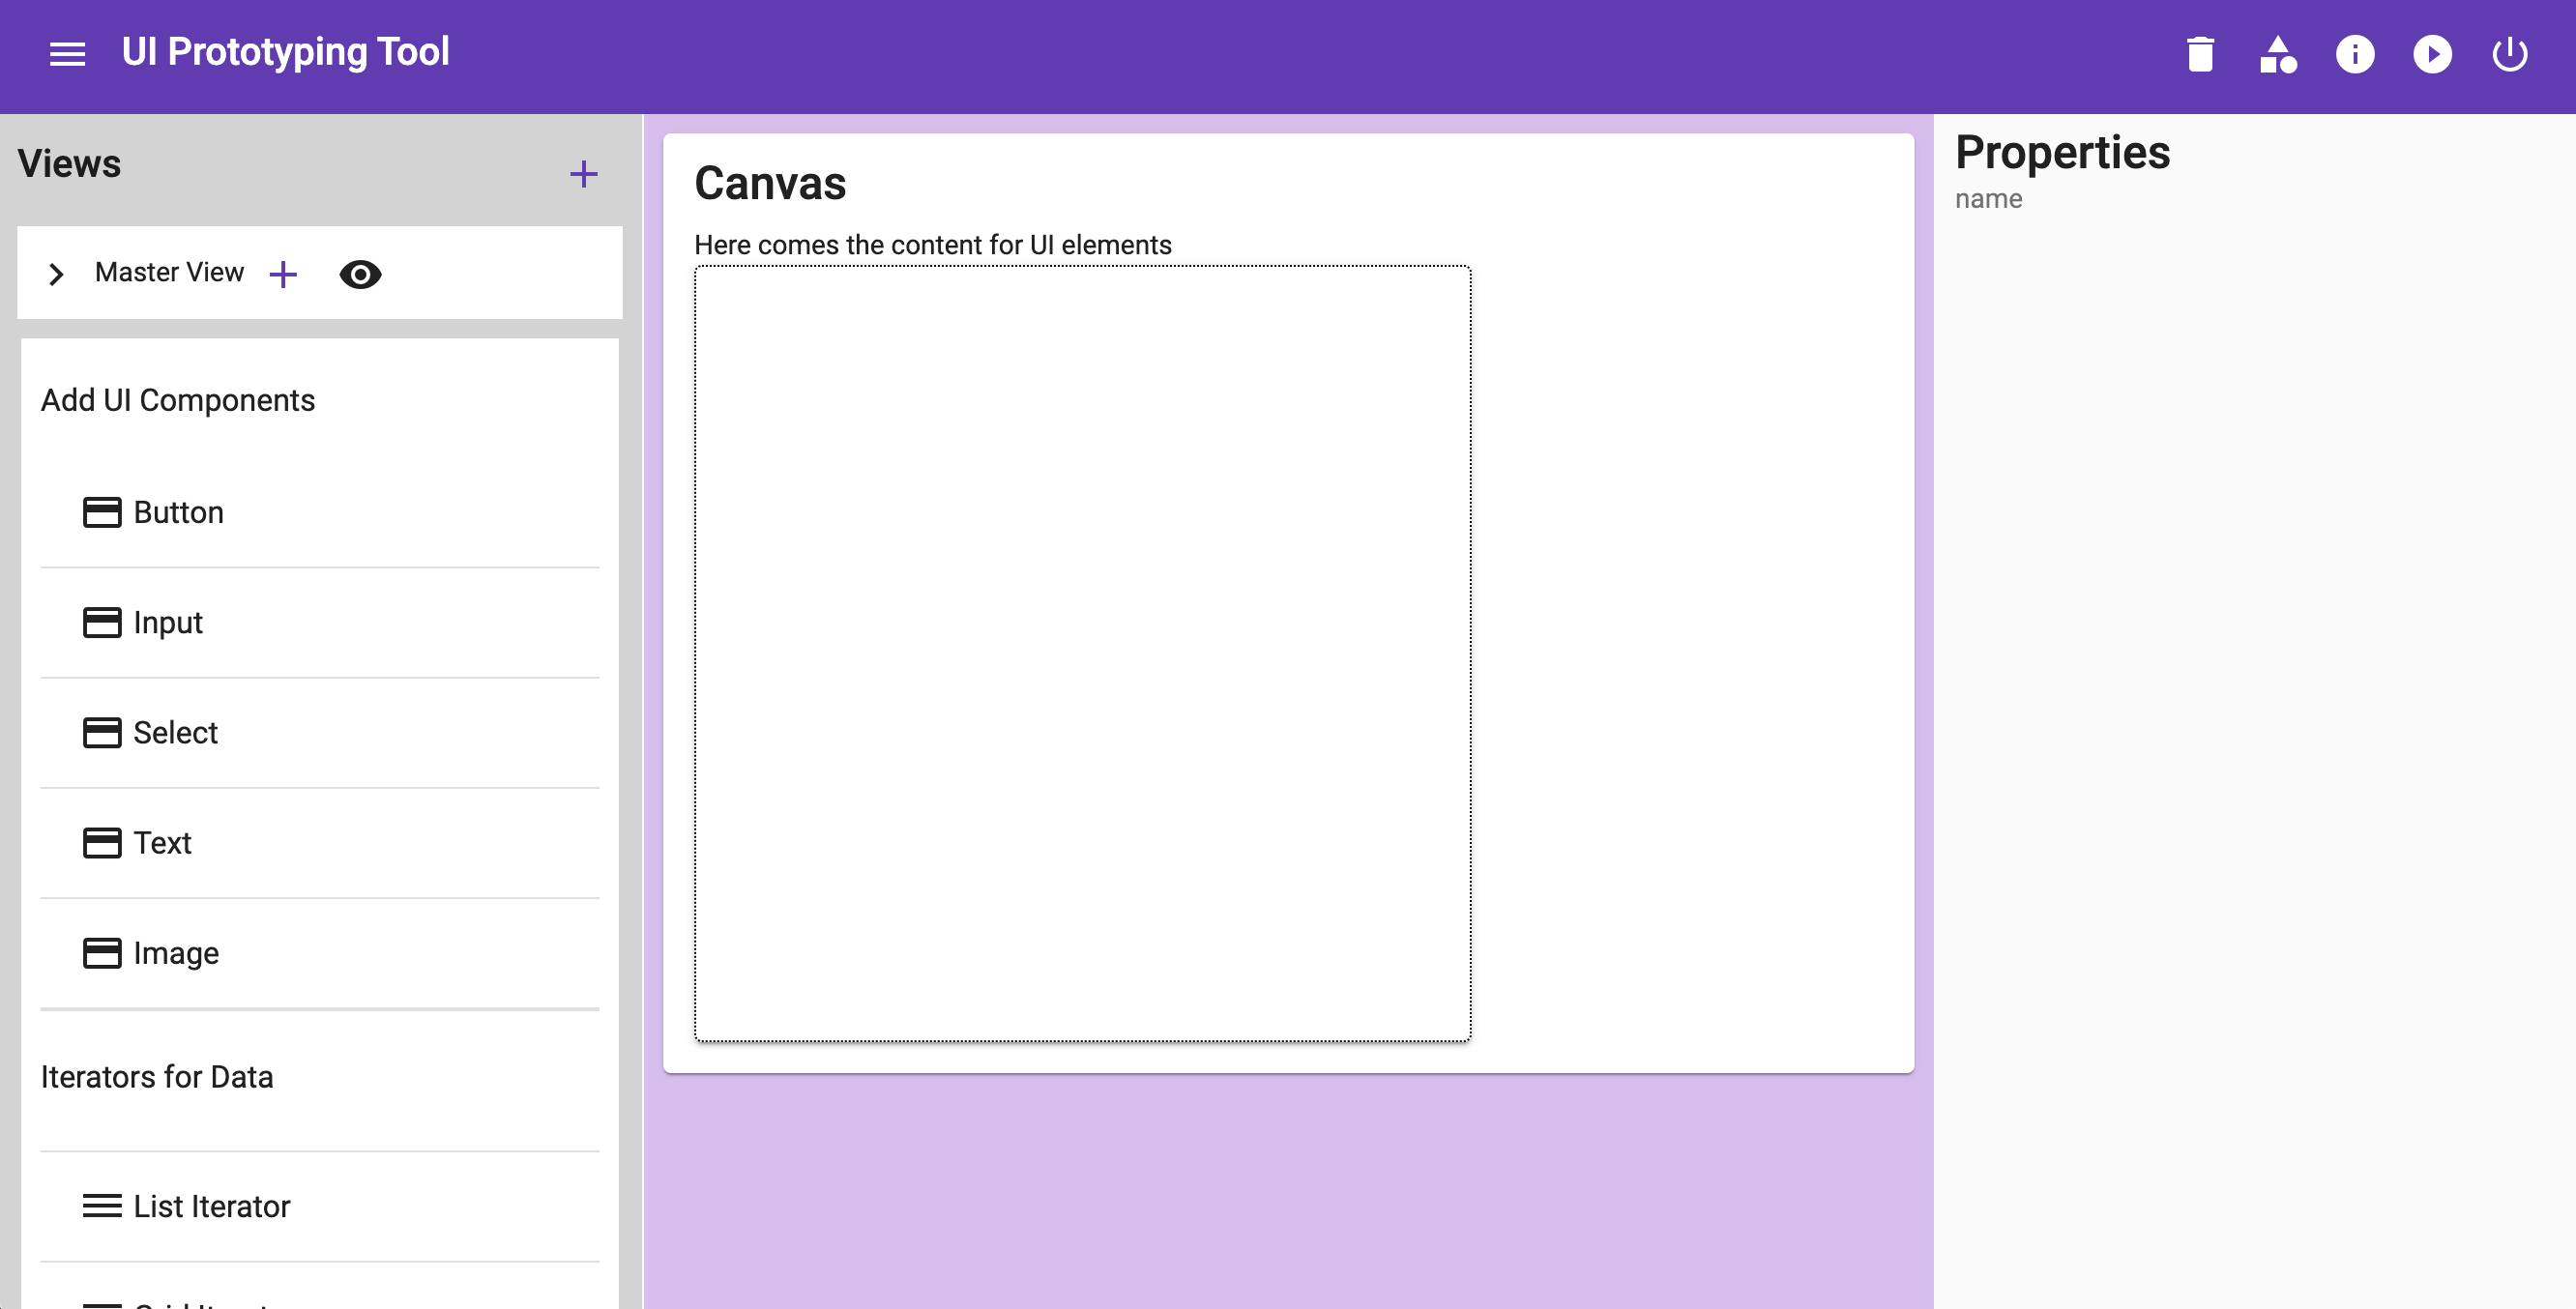
\includegraphics[width=0.8\textwidth]{tool.png}
	\caption[UI Prototyping tool]{Index page of our UI Prototyping tool}
	\label{fig:appendix:installation:tool}
\end{figure}
Lastly, for cloning the repository, you can install the Git\footnote{Website of Git installation: \url{https://git-scm.com/downloads}}.\\
Based on these prerequisites, there are additional instructions for installing the tool.

\begin{figure}[htbp]
	\begin{subfigure}[b]{0.55\textwidth}
	  \centering
	  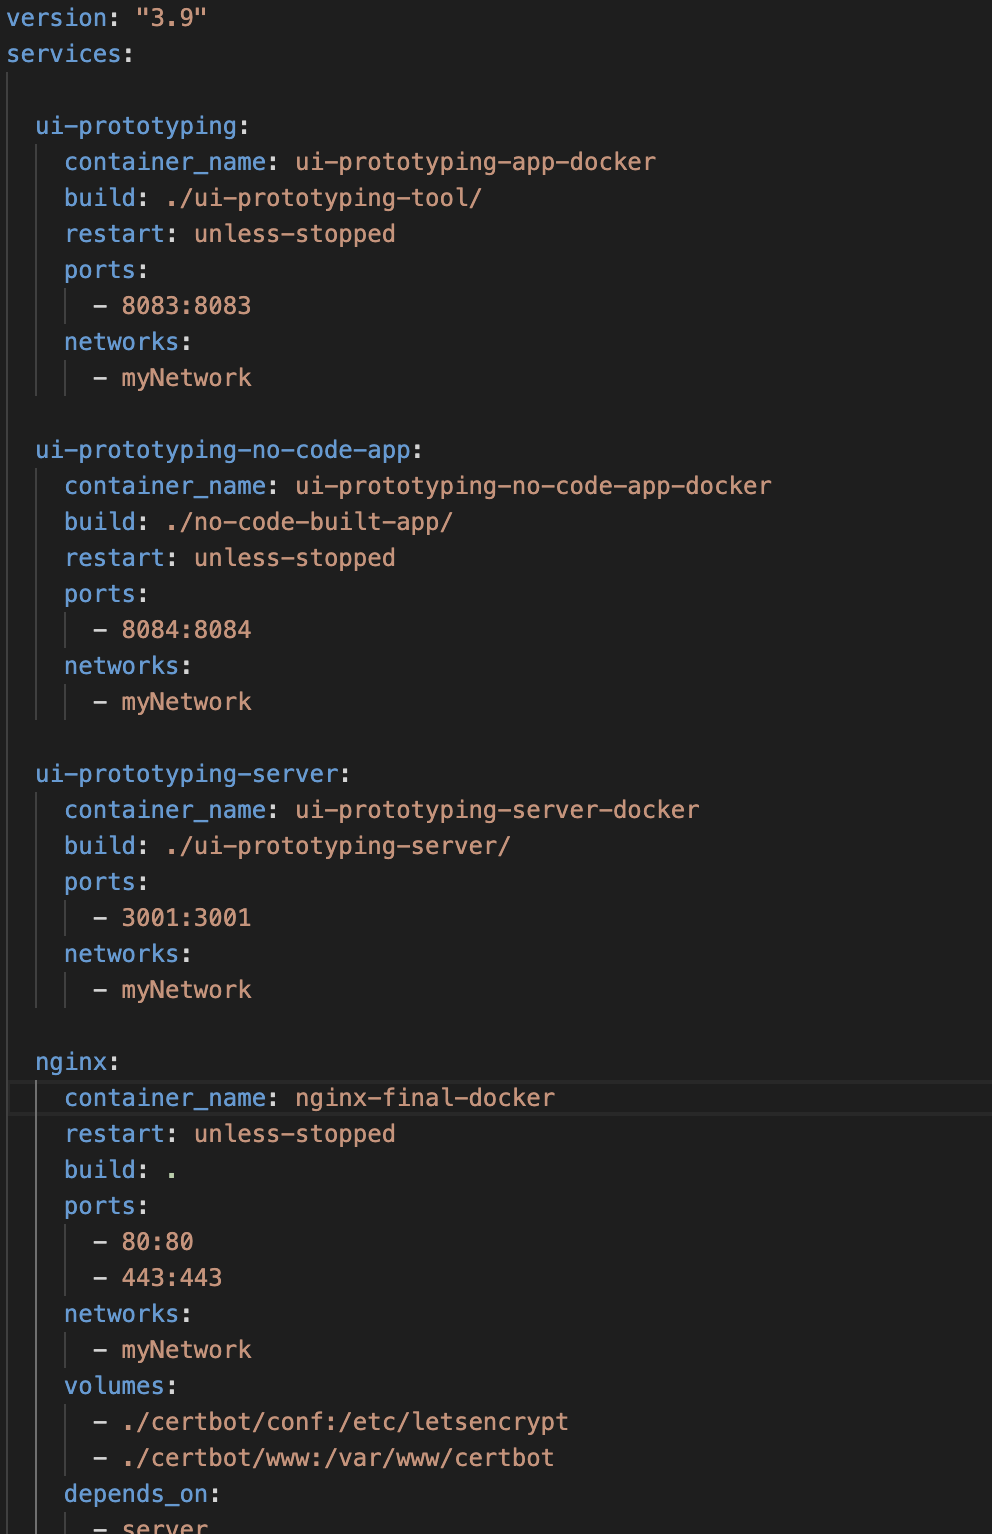
\includegraphics[width=1\textwidth]{docker-compose.png}
	\caption[Docker configuration]{A configuration file for docker-compose file}
	\label{fig:appendix:installation:dockerCompose}   
	\end{subfigure}
	\begin{subfigure}[b]{0.55\textwidth}
	  \centering
	  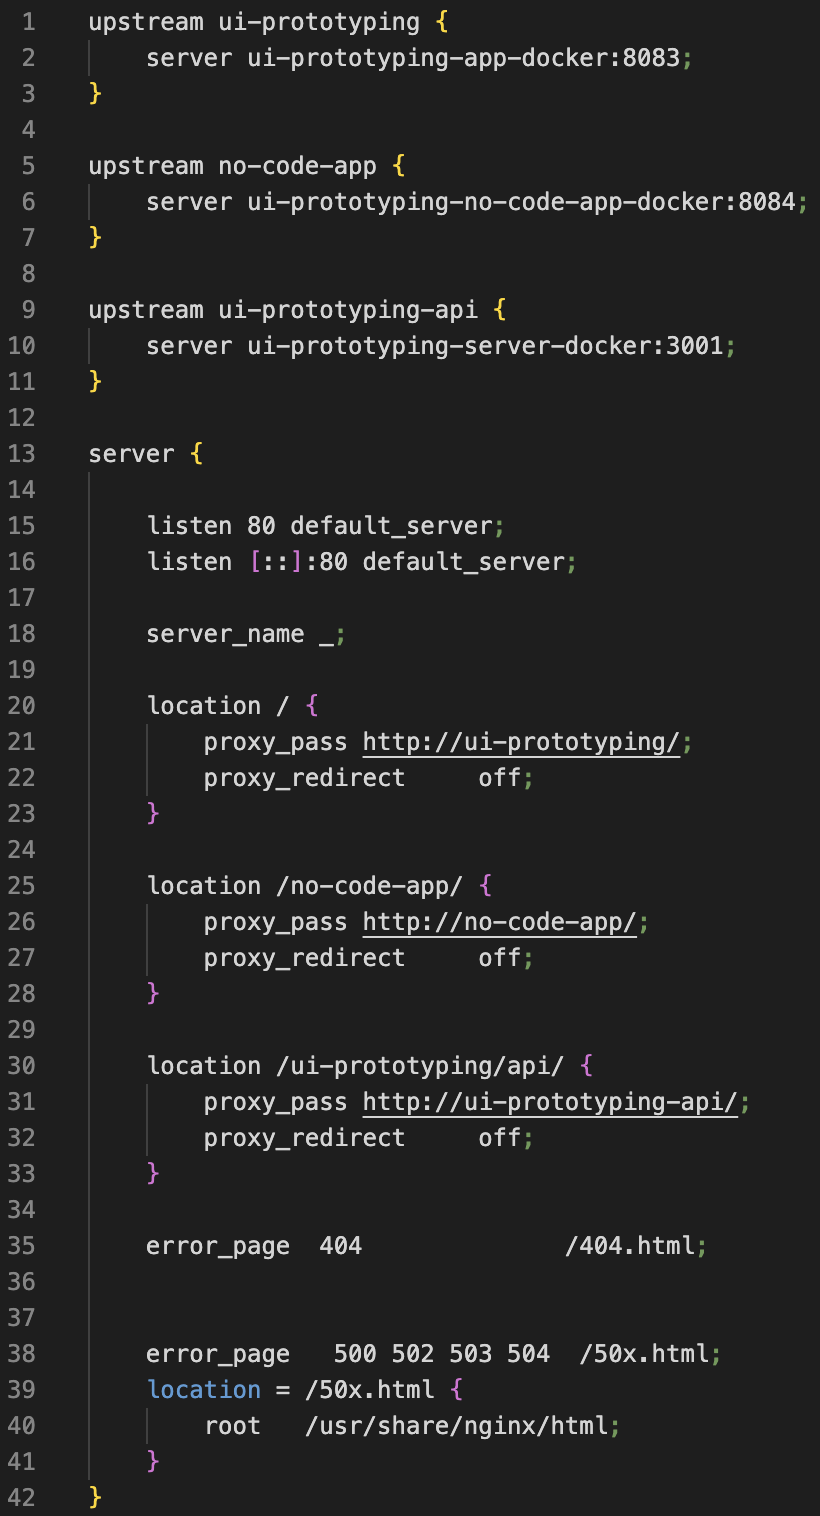
\includegraphics[width=0.838\textwidth]{nginx.png}
	\caption[Nginx Configuration]{Nginx Configuration for our tool}
	\label{fig:appendix:installation:nginx}
	\end{subfigure} 
	\caption{Configuration settings}
	\label{fig:appendix:configuration}
\end{figure}

\paragraph{Tool configuration steps:}

\begin{enumerate}
\item \textbf{Install Docker:} To begin with, you need to install Docker on your computer. 
You can download it from the official website\footnote{Website of Docker Installation: \url{https://www.docker.com/}} based on your operating system.
\clearpage
\item \textbf{Clone Repository:} Get the latest version of the tool from GitLab repository\footnote{Link for repo: \url{https://git.cs.uni-paderborn.de/rakshitb/thesis}}. We use GitLab which is hosted by the University of Paderborn.
\begin{enumerate}
	\item Clone the GitLab repository directly from GitLab\footnote{Website for cloning repository instructions: \url{https://docs.gitlab.com/ee/gitlab-basics/start-using-git.html}}.
	\item You can fork the repository\footnote{Website for forking a repository: \url{https://docs.gitlab.com/ee/user/project/repository/forking_workflow.html}} 
\end{enumerate}
% \begin{figure}[htbp!]
% 	\centering    
% 	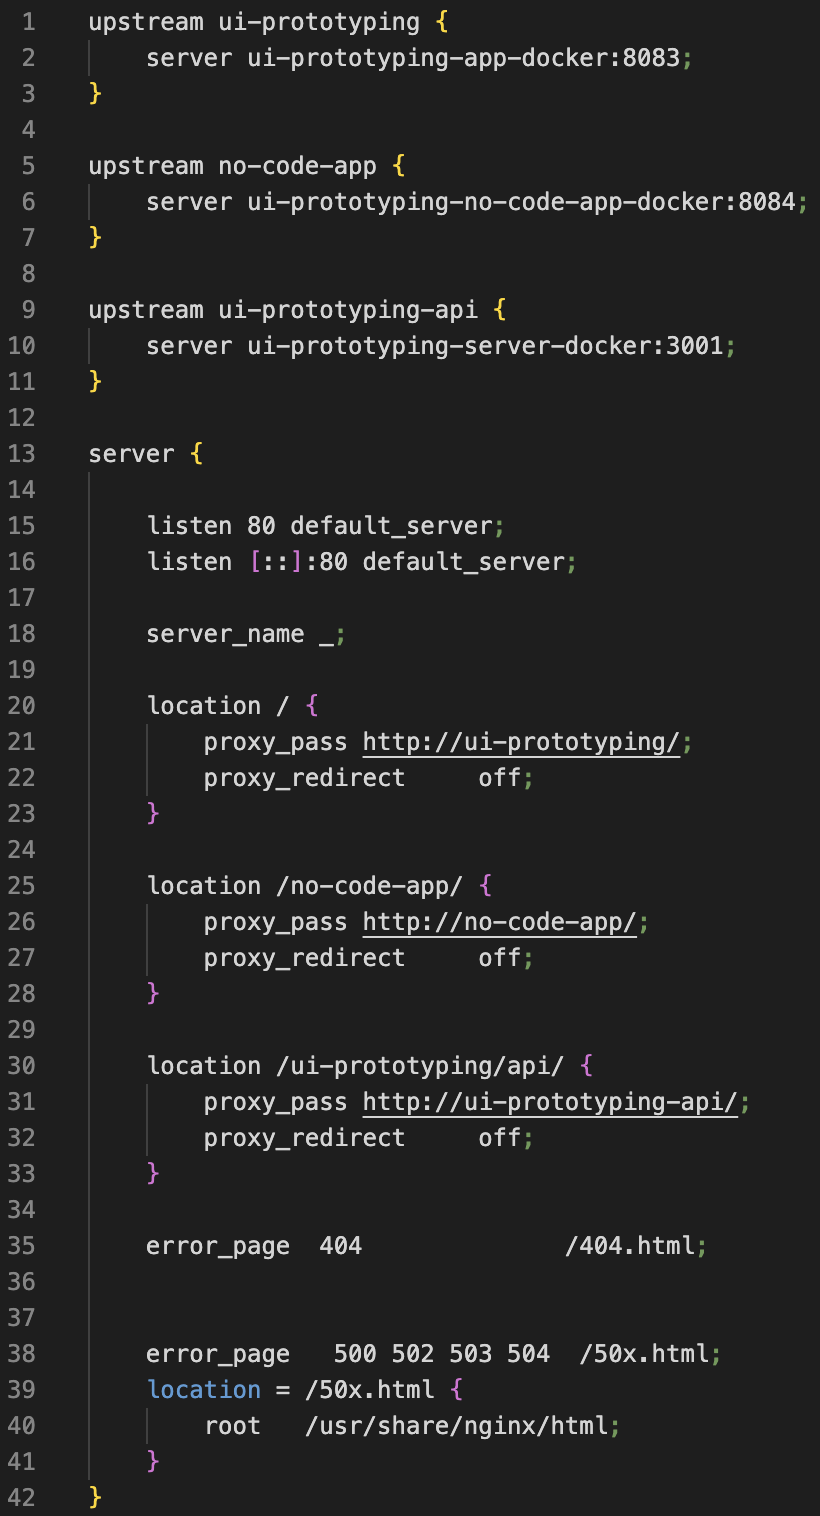
\includegraphics[width=0.4\textwidth]{nginx.png}
% 	\caption[Nginx Configuration]{Nginx Configuration for our tool}
% 	\label{fig:appendix:installation:nginx}
% \end{figure}
\item \textbf{Start docker daemon:} Start the docker engine or the service for running the docker containers\footnote{How to start docker deamon: \url{https://docs.docker.com/config/daemon/start/}}.
\item \textbf{Run Application:} Run the script file (\texttt{./restart-docker.sh}) which is available to run the docker containers. This also runs the \texttt{docker-compose.yml} file internally. You can update the file if you want to change the ports or add TLS signatures (see figure \ref{fig:appendix:installation:dockerCompose}).
\item \textbf{Check on Browser:} Use the UI Prototyping tool to develop the UI prototypes, create experiments and improve the prototype by opening \texttt{\url{http://localhost/}} in your web browser.
\end{enumerate}
%!TEX root = ../thesis.tex
% ******************************* Thesis Appendix B ********************************

\chapter{Literature Review topics and their references}
\label{appendix:two:definations}


\end{appendices}

% *************************************** Index ********************************
\printthesisindex % If the index is present

\end{document}
